\documentclass[11pt]{amsart}
%\documentclass[11pt]{article}
\usepackage{geometry}                % See geometry.pdf to learn the layout options. There are lots.
\geometry{letterpaper, width=7in, height=9in}                   % ... or a4paper or a5paper or ... 
\usepackage{graphicx}
\usepackage{pdfpages}
\usepackage{amssymb}
\usepackage{epstopdf}
\usepackage{color}
\usepackage{hyperref}
\usepackage{courier}
\usepackage{listings}
%\usepackage[titles]{tocloft}

\usepackage{siunitx}
\usepackage{booktabs}

\let\oldsection\section
\renewcommand\section{\clearpage\oldsection}

\DeclareGraphicsRule{.tif}{png}{.png}{`convert #1 `dirname #1`/`basename #1 .tif`.png}
\DeclareGraphicsRule{.gif}{pdf}{.pdf}{`convert #1 `dirname #1`/`basename #1 .gif`.pdf}

   \newsavebox{\fmbox}
   \newenvironment{fmpage}[1]
     {\begin{lrbox}{\fmbox}\begin{minipage}{#1}}
     {\end{minipage}\end{lrbox}\fbox{\usebox{\fmbox}}}
     
\oddsidemargin 0in
\evensidemargin 0in

\definecolor{MRGGreen}{rgb}{0,0.655,0.212}
\parskip 10pt
\parindent 0em

\lstset{columns=fullflexible, basicstyle=\ttfamily, xleftmargin=0.5cm, frame=tlbr,framesep=4pt, framerule=0pt}

%\usepackage[nottoc]{tocbibind}
%\usepackage[colorlinks=true,linkcolor=blue]{hyperref}
%\setcounter{tocdepth}{0}

%\cftsetindents{section}{0em}{2.3em}
%\cftsetindents{subsection}{0em}{4.3em}

\begin{document}

\begin{center}

\includegraphics[height=0.75in]{graphics/logo.pdf}\\
\textcolor{MRGGreen}{\sf
\begin{tabbing}
Metrum Research Group LLC \` 2 Tunxis Road, Suite 112 \\
Phone: 860.735.7043 \` Tariffville, CT 06081 \\
charlesm@metrumrg.com \` metrumrg.com \\
\end{tabbing}
}
{\Huge \textbf{Torsten} \\ \ \\  \huge A Prototype Library for Bayesian Pharmacometrics Modeling in Stan \\ \ \\
User Manual \\ \ \\ 
\Large Charles Margossian and Bill Gillespie \\ \ \\ \ \\ \ \\ \ \\
Torsten Version 0.82 \\ for Stan Version 2.14.0 \\ \ \\ 
\large Tuesday January 31st 2017 }
\end{center}

\clearpage

\tableofcontents
%\addtocontents{toc}{~\hfill\textbf{Page}\par}

\section*{Aknowledgements}

{\bf Institutions} \ \\
We thank Metrum Research Group, Columbia University, and AstraZeneca.

{\bf Grants}
\begin{itemize}
  \item Small Business Technology Transfer from the Office of Naval Research: funds collaboration between Columbia University and Metrum Research Group for the development of tools for \textit{Fast and Flexible Differential Equation Model Fitting with Application to Pharmacometrics}.
  \item  Bill and Melinda Gates foundation grant for the \textit{Development of a Pharmacometrics Library for Stan}
\end{itemize}

{\bf Individuals} \ \\
A very special thank to the Stan Development Team for creating Stan, building new mathematical tools with applications in, among other fields, Pharmacometrics, and their support for Torsten. We also thank Kyle Baron and Hunter Ford for helpful advice on coding in C++ and using GitHub, and Curtis Johnston for reviewing the User Manual. 

\section{Introduction}
%\addcontentsline{toc}{section}{Introduction}

\subsection{Preface} \ \\ \ \\ Stan is an open source probabilistic language designed primarily to do Bayesian data analysis \cite{stan}. Several of its features make it a powerful tool to specify and fit complex models. Notably, its language is extremely flexible and its No U-Turn Sampler (NUTS), an adaptative Hamiltonian Monte Carlo algorithm, has proven more efficient than commonly used Monte Carlo Markov Chains (MCMC) samplers for complex high dimensional problems \cite{nuts}. Our goal is to harness these innovative features and make Stan a better software for pharmacometrics modeling. Our efforts are twofold:
\begin{enumerate}
  \item We contribute to the development of new mathematical tools, such as functions that support differential equations based models, and implement them directly into Stan's core language.
  \item We develop Torsten, an extension with specialized pharmacometrics functions.
\end{enumerate}

Throughout the process, we have been working very closely with Stan's development team. We have benefited immensely from their mentoring, advice, and feedback. Just like Stan, Torsten is an open source project that fosters collaborative work. Interested in contributing? Shoot us an e-mail and we will help you help us (\url{charlesm@metrumrg.com} and \url{billg@metrumrg.com})!

Torsten is licensed under the BSD 3-clause license.

\begin{fmpage}{\textwidth}
{\bf WARNING:} The current version of Torsten is a {\em prototype}. It is being released for review and comment, and to support limited research applications. It has not been rigorously tested and should not be used for critical applications without further testing or cross-checking by comparison with other methods. \\ \ \\
We encourage interested users to try Torsten out and are happy to assist. Please report issues, bugs, and feature requests on our GitHub page: \url{https://github.com/charlesm93/stan}.
\end{fmpage}

\subsection{Installing Torsten}  \ \\ \ \\  
Installation files are available on GitHub: \url{https://github.com/charlesm93/example-models/tree/torsten-0.82/PKPD/torsten}

There is currently no mechanism to install Torsten on top of your version of Stan. This is still a work in progress. In the meantime, we offer a version of Stan with Torsten built inside of it. Torsten 0.82 works with Stan 2.14.0. Torsten is built inside the Stan and Stan-math repositories and is agnostic to the interface the users use. We offer support for installing Stan with CmdStan\footnote{If you need assistance to set up Torsten with another interface, shoot me an e-mail at charlesm@metrumrg.com. I'm happy to help.}.

The easiest way to install the CmdStan interface with Stan and Torsten is to run the bash file \texttt{setupTorsten.sh}. You can also do it manually on a terminal window:

Download CmdStan: \\
\texttt{git clone https://github.com/stan-dev/cmdstan.git \\
cd cmdstan \\
git checkout release/v2.14.0
} \\

Download Stan with Torsten: \\
\texttt{git clone https://github.com/charlesm93/stan.git \\
rm -r stan\_2.14.0 \\
mv stan stan\_2.14.0 \\
cd stan\_2.14.0 \\
git checkout torsten-master
} \\

Download Stan\_math with Torsten:
\texttt{cd lib \\
git clone https://github.com/charlesm93/math.git \\
mv math stan\_math\_2.14.0 \\
cd stan\_math\_2.14.0 \\
git checkout torsten-master
}

\subsection{Overview} \ \\ \ \\
Torsten is a prototype Pharmacokinetic/Pharmacodynamic (PKPD) model library for use in Stan 2.14.0. The current version includes:
\begin{itemize}
  \item Specific linear compartmental models:
  \begin{itemize}
    \item One compartment model with first order absorption
    \item Two compartment model with elimination from and first order absorption into central compartment
  \end{itemize}
  \item General linear compartmental model described by a system of first-order linear Ordinary Differential Equations (ODEs).
  \item General compartmental model described by a system of first order ODEs 
 \end{itemize}

The models and data format are based on NONMEM\textregistered\footnote{NONMEM\textregistered\ is licensed and distributed by ICON Development Solutions.}/NMTRAN/PREDPP conventions including:
\begin{itemize}
  \item Recursive calculation of model predictions
  \begin{itemize}
    \item This permits piecewise constant covariate values
  \end{itemize}
  \item Bolus or constant rate inputs into any compartment
  \item Handles single dose and multiple dose histories
  \item Handles steady-state dosing histories for specific and general \underline{linear} models
  \item Implemented NMTRAN data items include: TIME, EVID, CMT, AMT, RATE, ADDL, II, SS
\end{itemize}

This library provides Stan language functions that calculate amounts in each compartment, given an event schedule and an ODE system.
    
\subsection{Implementation details}
\begin{itemize}
  \item Stan version 2.14.0 (\url{http://mc-stan.org/})
  \item All functions are programmed in C++ and are compatible with the Stan-math automatic differentiation library \cite{AD}
  \item All functions can be called directly in a Stan file in a manner identical to other built-in functions
  \item One and two compartment models: hand-coded analytical solutions
  \item General linear compartment models with semi-analytical solutions using a built-in Matrix Exponential function (Pade approximation coupled with scaling and squaring \cite{matrixExp})
  \item General compartment models with numerical solutions to ODEs using built-in ODE integrators in Stan (Runge-Kutta 4th/5th and backward differentiation methods from CVODES library), with adjustable tuning parameters
\end{itemize}



\subsection{Development plans} \ \\ \ \\
Our current plans for future development of Torsten include the following:
\begin{itemize}
  \item A system to easily share packages of Stan functions (written in C++ or in the Stan language)
  \item Steady state calculation for the General compartment model
  \begin{itemize}
    \item This requires a solver for nonlinear algebraic equations (aka a root solver)
  \end{itemize}
  \item Optimize Matrix exponential functions
  \begin{itemize}
    \item Function for the action of Matrix Exponential on a vector
    \item Hand-coded gradients
    \item Special algorithm for matrices with special properties
  \end{itemize}
  \item Fix issue that arises when computing the adjoint of the lag time parameter (in a dosing compartment) evaluated at $t_{lag} = 0$. 
  \item Make the following arguments optional
  \begin{itemize}
    \item \texttt{biovar} and \texttt{tlag}, respectively used for the bioavailability fraction and the lag times in each compartment
    \item Tuning parameters of the ODE integrators for the general compartmental function.
  \end{itemize}
  \item Extend formal tests
  \begin{itemize}
    \item We want more C++ Google unit tests to address cases users may encounter 
    \item Comparison with simulations from the R package \textit{mrgsolve} and the software NONMEM\textregistered
    \item Recruit non-developer users to conduct beta testing
  \end{itemize}
\end{itemize}

\subsection{Updates since Torsten 0.81}
\begin{itemize}
  \item Torsten is now up to date with Stan version 2.14.0
  \item We split the parameter argument into three arguments: \texttt{pMatrix} (parameters for ODEs), \texttt{biovar} (parameters for the bioavailability), and \texttt{tlag} (parameters for lag times). This gives the users more control over which arguments get passed as data and as parameters. The model is most efficient when all fixed values are passed as data.
  \item We changed the order of the arguments: the user first passes the data arguments and then the parameter arguments. This is because in future versions we will want optional arguments to be passed last.
  \item The user can now pass parameter arguments as 1D or 2D arrays, depending on whether the parameters are constant or change from one event to the other.
  \item We have significantly increased the number of unit tests -- but we still have more to do!
  \item The unit tests now check automatic differentiation against finite differentiation calculations.
  \item Fixed minor bugs and report issues.
\end{itemize}
 


\section{Using Torsten}

The reader should have a basic understanding of how Stan works before tackling this chapter. There are excellent resources online to get started with Stan (\url{http://mc-stan.org/documentation/}). 

In this section we go through the different functions Torsten adds to Stan. It will be helpful to apply these functions to a simple example. We have uploaded code and data on \url{https://github.com/charlesm93/example-models/tree/torsten-0.82/PKPD/torsten}.

\subsection{Example 1: Two Compartment Model}
We model drug absorption in a single patient and simulate plasma drug concentrations:
\begin{itemize}
  \item Single Dose: 5000 mg
  \item PK: plasma concentrations of parent drug ($c$)
  \item PK measured at 0, 0.25, 0.50, 0.75, 1, 1.25, 1.50, 1.75, 2, 4, 6, 8, 10, 12, 14, 16, 18, and 20 hours after dosing
\end{itemize}

The plasma concentration ($c$) are simulated according to the following equations:
\begin{eqnarray*}
\log\left(c\right) &\sim& N\left(\log\left(\widehat{c}\right),\sigma^2\right) \\
 \widehat{c} &=& f_{2cpt}\left(t, CL, Q, V_2, V_3, k_a\right) \\
  \left(CL, Q, V_2, V_3, ka\right) &=& 
	\left(5\ {\rm L/h}, 8\  {\rm L/h}, 20\  {\rm L},  70\ {\rm L}, 1.2\ {\rm h^{-1}} \right) \\
  \sigma &=& 0.05
\end{eqnarray*}

The data are generated using the R package \textit{mrgsolve}\footnote{https://github.com/metrumresearchgroup/mrgsolve}, see \texttt{TwoCptModelSimulation.R}. We show the results obtained when using the function \texttt{PKModelTwoCpt}, which computes solutions to the ODEs analytically.

\subsection{Linear One and Two Compartment Model Function} \ \\

The one and two compartment model functions have the form:

\texttt{<model name>(time, amt, rate, ii, evid, cmt, addl, ss,\\
\phantom{<model name>} theta,  biovar, tlag)} \\

There is no need to skip a line, but we do so to separate what we call \textit{event} arguments and \textit{model} arguments. The event arguments describe the event schedule of the clinical trial. \texttt{time, amt, rate, ii} are arrays of real and \texttt{evid, cmt, addl, ss} arrays of integers. All arrays have the same length, which corresponds to the number of events.

Next we have the \textit{model} arguments: \texttt{theta} contains the ODE parameters, \texttt{biovar} the bioavailability fraction in each compartment (sometimes denoted as \textit{F} and called \textit{biovariability}), and \texttt{tlag} the lag times in each compartment. The model arguments are 2-dimensional arrays. The first dimension provides a container for the parameters and the length of that container is simply the number of parameters. The second dimension allows for variations in the parameters from one event to the other. The length of the 2D container is the number of events. The \textit{ith} row contains an array of parameters for the time interval [\texttt{time[i-1], time[i]}]. Often times, the parameters are constant for all events and the user can then pass a 2D array of length 1 or, even better, a 1D array.

The options for \textit{model name} are:
\begin{itemize}
  \item PKModelOneCpt
  \item PKModelTwoCpt
\end{itemize}
which respectively correspond to the one and two compartment model with first order absorption (figure~\ref{cptModels}). A vector in \texttt{theta} is expected to contain parameters $CL$, $V2$, and $ka$ for the one compartment case, and $CL$, $Q$, $V2$, $V3$, and $ka$ for the two compartments case, \underline{in this order}. Setting $ka$ to 0 eliminates the fist-order absoprtion. \texttt{biovar} contains the bioavailability fraction of each compartment (non-effective if set to 1) and \texttt{tlag} the lag time in each compartment (non-effective if set to 0).

\begin{figure}[htbp]
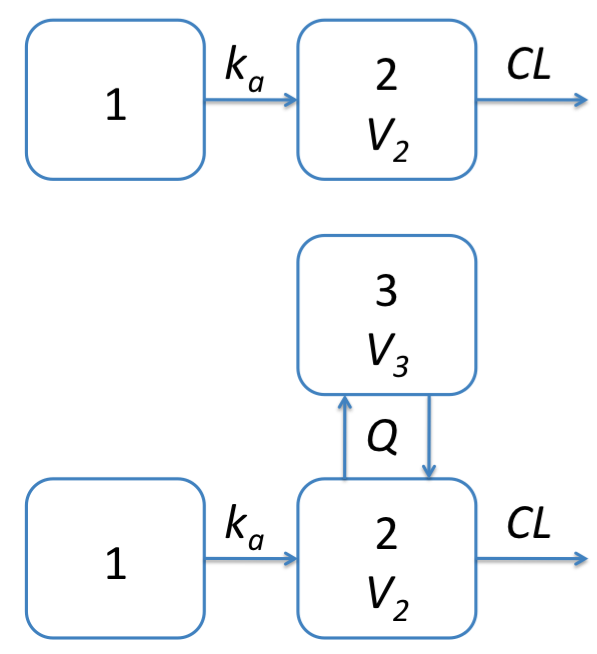
\includegraphics[width=3.5in,trim=0in 0in 0 0in]{graphics/cptModels.png}
\caption{One and two compartment models with first order absorption implemented in Torsten.}
\label{cptModels}
\end{figure}

\texttt{PKModelTwoCpt} can be used to fit example 1, see \texttt{TwoCptModel.stan}. We are interested in evaluating the ODE parameters, stored in \texttt{theta}. The bioavailability fraction and the lag times on the other hand are fixed, and we therefore declare \texttt{biovar} and \texttt{tlag} in the transformed data block. Four MCMC chains of 2000 iterations were simulated. The first 1000 iteration of each chain were discarded. Thus 1000 MCMC samples were used for the subsequent analyses.

\begin{figure}[htbp]
\caption{Stan language for fitting a two compartment model using the \texttt{PKModelTwoCpt} function (abstract)}
\begin{center}
\begin{small}
\begin{fmpage}{\textwidth - .75in}
\begin{lstlisting}[basicstyle=\footnotesize\ttfamily,mathescape=true,flexiblecolumns=true,frame=single,escapeinside=`']
`\bf{data}' {
  int<lower = 1> nt; `\textcolor{gray}{\# number of events}'
  int<lower = 1> nObs; `\textcolor{gray}{\# number of observation}'
  int<lower = 1> iObs[nObs]; `\textcolor{gray}{\# index of observation}'
  int<lower = 1> cmt[nt];
  int evid[nt];
  int addl[nt];
  int ss[nt];
  real amt[nt];
  real time[nt];
  real rate[nt];
  real ii[nt];
  
  vector<lower = 0>[nObs] cObs; `\textcolor{gray}{\#  observed concentration (Dependent Variable)}'
}

`\bf{transformed data}' {
                                    $\vdots$
  biovar[1] = 1;
  biovar[2] = 1;
  biovar[3] = 1;
  
  tlag[1] = 0;
  tlag[2] = 0;
  tlag[3] = 0;                                    
                                    
                                     
}
                                    $\vdots$ 
`\bf{parameters}' {
  real<lower = 0> CL;
  real<lower = 0> Q;
  real<lower = 0> V2;
  real<lower = 0> V3;
  real<lower = 0> ka;
  real<lower = 0> sigma;
}

`\bf{transformed parameters}' {
                                    $\vdots$ 
  theta[1] = CL;
  theta[2] = Q;
  theta[3] = V2;
  theta[4] = V3;
  theta[5] = ka;

  x = `\textcolor{red}{PKModelTwoCpt}'(time, amt, rate, ii, evid, cmt, addl, ss, 
                          theta, biovar, tlag);

  cHat = col(x, 2) ./ V2; `\textcolor{gray}{\#  get concentration in the central compartment}'

  for(i in 1:nObs){
    cHatObs[i] = cHat[iObs[i]];`\textcolor{gray}{\# predictions for observed data records}'
  }
 }
                                    $\vdots$ 
\end{lstlisting}
\end{fmpage}
\end{small}
\end{center}
\label{TwoCptCode}
\end{figure}

\textbf{Result.} The MCMC history plots (figure~\ref{TwoCptMCMC}) suggest that the 4 chains have converged to common distributions for all of the key model parameters. The  fit to the plasma concentration data (figure~\ref{TwoCptPredictions}) are in close agreement with the data, which is not surprising since the fitted model is identical to the one used to simulate the data. Similarly the parameter estimates summarized in Table 1 are consistent with the values used for simulation.

\begin{figure}[htbp]
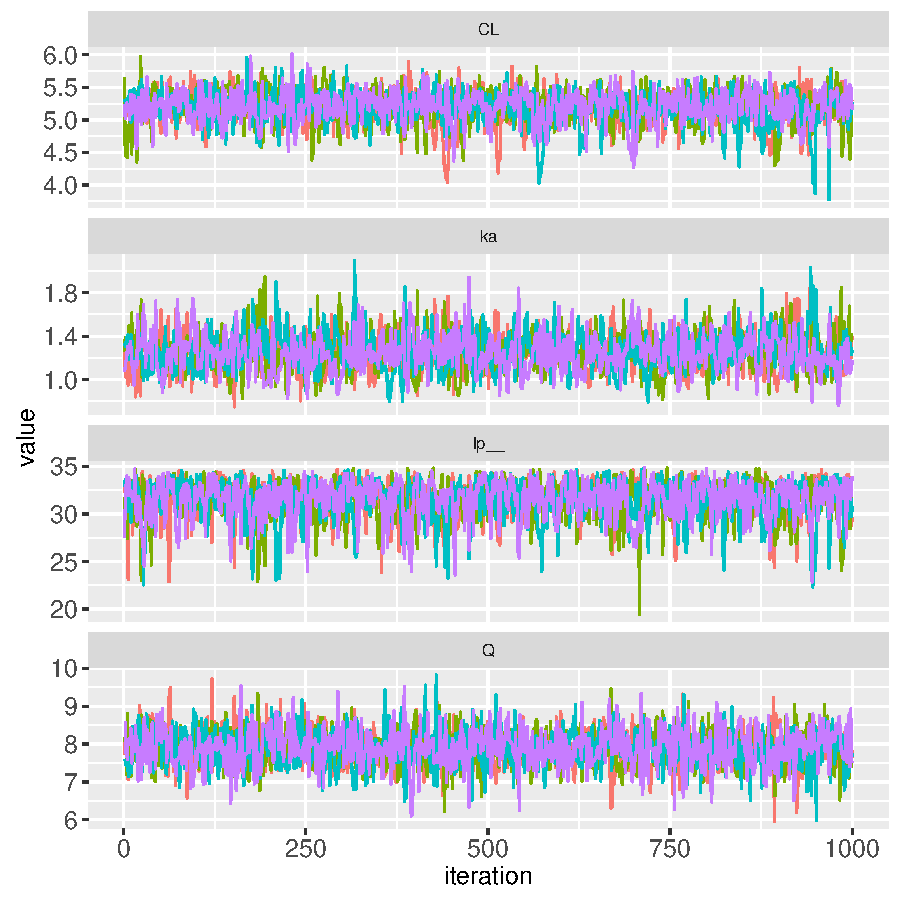
\includegraphics[width=3.0in,trim=0in 0in 0 0in]{graphics/TwoCptModelExamplePlots001.pdf}
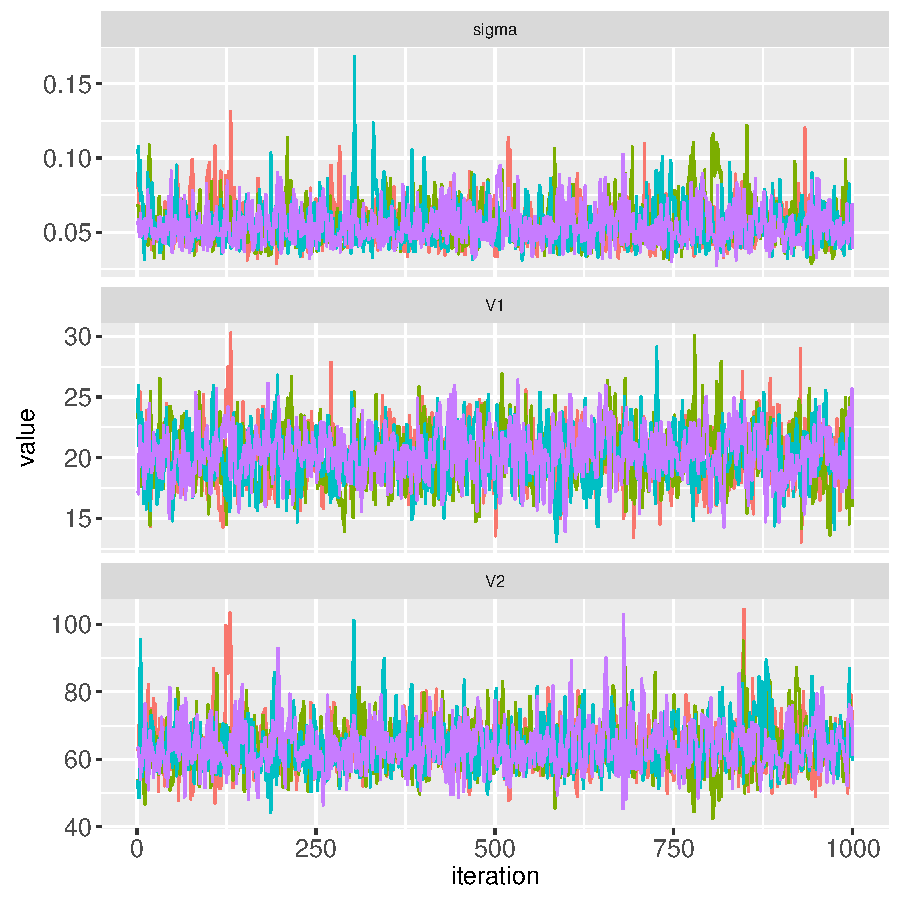
\includegraphics[width=3.0in,trim=0in 0in 0 0in]{graphics/TwoCptModelExamplePlots002.pdf}
\caption{{MCMC history plots for the parameters of a two compartment model with first order absorption (each color corresponds to a different chain)}}
\label{TwoCptMCMC}
\end{figure}

\begin{figure}[!htb]
\begin{center}
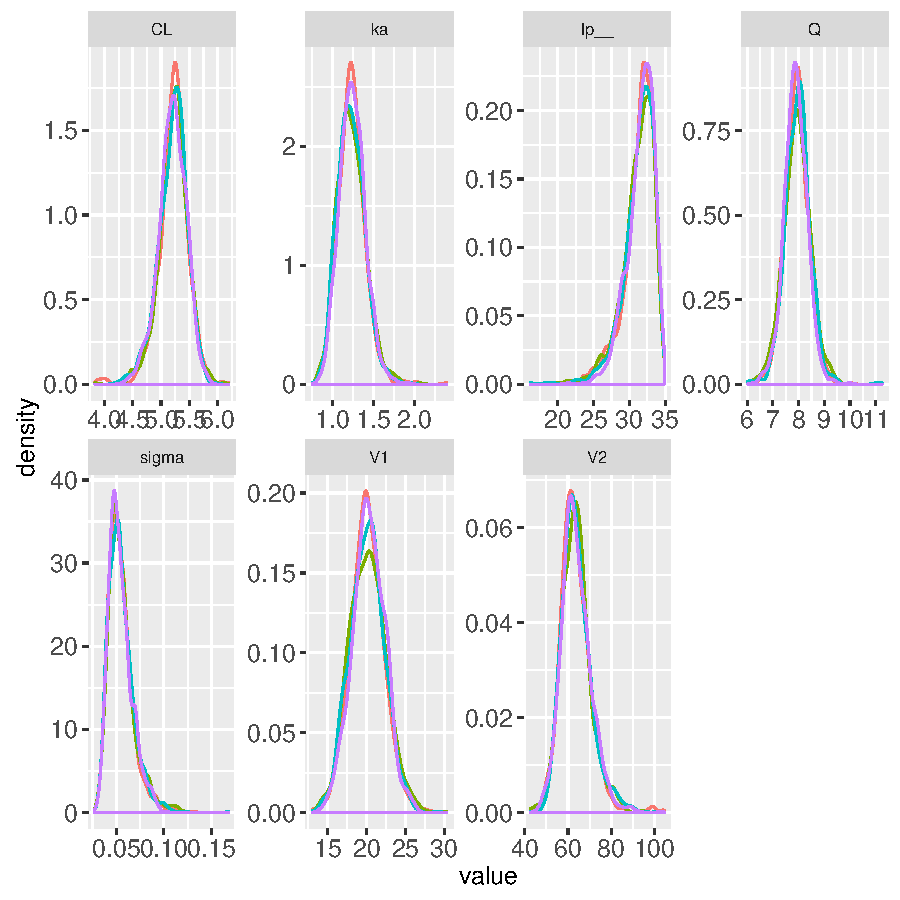
\includegraphics[width=4.5in,trim=0in 0in 0 0in]{graphics/TwoCptModelExamplePlots004.pdf}
\caption{{Posterior Marginal Densities of the Model Parameters of a two compartment model with first order absorption (each color corresponds to a different chain)}}
\label{TwoCptDensity}
\end{center}
\end{figure}

\begin{figure}[!htb]
\begin{center}
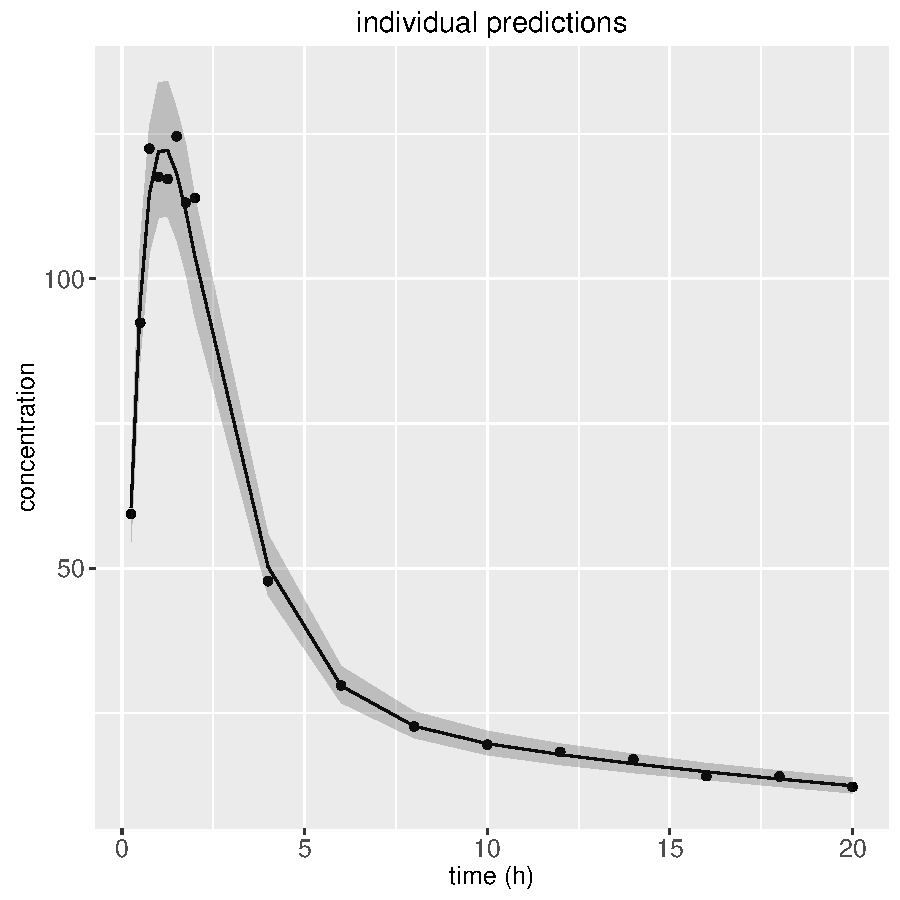
\includegraphics[width=3.5in,trim=0in 0in 0 0in]{graphics/TwoCptModelExamplePlots006.pdf}
\caption{{Predicted (posterior median and 90 \% credible intervals) and observed plasma drug concentrations of a two compartment model with first order absorption}}
\label{TwoCptPredictions}
\end{center}
\end{figure}

\begin{table}[!htb]
\centering
\caption{Summary of the MCMC simulations of the marginal posterior distributions of the model parameters}
\begin{tabular}{rrrrrrrrrrr}
  \hline
 & mean & se\_mean & sd & 2.5\% & 25\% & 50\% & 75\% & 97.5\% & n\_eff & Rhat \\ 
  \hline
CL & 5.19 & 0.01 & 0.25 & 4.60 & 5.05 & 5.21 & 5.35 & 5.62 & 971.04 & 1.00 \\ 
  Q & 7.90 & 0.01 & 0.47 & 6.97 & 7.58 & 7.93 & 8.21 & 8.79 & 1662.02 & 1.00 \\ 
  V2 & 20.25 & 0.08 & 2.27 & 15.71 & 18.74 & 20.23 & 21.76 & 24.67 & 896.67 & 1.00 \\ 
  V3 & 64.10 & 0.22 & 6.98 & 52.60 & 59.48 & 63.38 & 67.74 & 80.65 & 1032.66 & 1.00 \\ 
  ka & 1.25 & 0.00 & 0.17 & 0.94 & 1.13 & 1.24 & 1.35 & 1.62 & 940.99 & 1.00 \\ 
   \hline
\end{tabular}
\end{table}

\subsection{General Linear ODE Model Function} \ \\

A general linear ODE model refers to a model that may be described in terms of a system of first order linear differential equations with (piecewise) constant coefficients, i.e., a differential equation of the form:
$$ y^\prime\left(t\right) = Ky\left(t\right) $$
where $K$ is a matrix. For example $K$ for a two compartment model with first order absorption is:
$$   K = \left[\begin{array}{ccc}
	-k_a & 0 & 0 \\
	k_a & -\left(k_{10} + k_{12}\right) & k_{21} \\
	0 & k_{12} & -k_{21}
	\end{array}\right] $$ \\
where $k_{10} = CL / V2 $, $ k_{12} = Q / V2 $, and $k_{21} = Q / V2 $.

The linear ODE model function has the form:

\texttt{linOdeModel(time, amt, rate, ii, evid, cmt, addl, ss,\\
\phantom{linOdeModel} system, biovar, tlag)}

where \texttt{system} is an array of constant rate matrices. The length of the array is the number of events. If the rate matrix is constant for all events, the user may pass an array of length 1 or directly the matrix \texttt{K}.  \texttt{system} contains all the ODE parameters, so we no longer need \texttt{theta}.

\begin{figure}[!htb]
\caption{Stan language for fitting a two compartment model using the \texttt{linOdeModel} function (abstract)}
\begin{center}
\begin{small}
\begin{fmpage}{\textwidth - .75in}
\begin{lstlisting}[basicstyle=\footnotesize\ttfamily,mathescape=true,flexiblecolumns=true,frame=single,escapeinside=`']
`\bf{transformed parameters}' {
  `\textcolor{red}{matrix[3, 3] K;}'
  real k10 = CL / V2;
  real k12 = Q / V2;
  real k21 = Q / V3;
  vector<lower = 0>[nTheta] theta[1];
  vector<lower = 0>[nt] cHat;
  vector<lower = 0>[nObs] cHatObs;
  matrix<lower = 0>[nt, 3] x;
 
  `\textcolor{red}{K = rep\_matrix(0, 3, 3);}'

  `\textcolor{red}{K[1, 1] = -ka;}'  
  `\textcolor{red}{K[2, 1] = ka;}' 
  `\textcolor{red}{K[2, 2] = -(k10 + k12);}' 
  `\textcolor{red}{K[2, 3] = k21;}' 
  `\textcolor{red}{K[3, 2] = k12;}' 
  `\textcolor{red}{K[3, 3] = -k21;}'

  x = `\textcolor{red}{linOdeModel}'(time, amt, rate, ii, evid, cmt, addl, ss,
                       K, biovar, tlag);

  cHat = col(x, 2) ./ V1;

  for(i in 1:nObs){
    cHatObs[i] = cHat[iObs[i]]; `\textcolor{gray}{\# predictions for observed data records}'
  }
}

`\bf{model}'{
  logCObs ~ normal(log(cHatObs), sigma);
}
\end{lstlisting}
\end{fmpage}
\end{small}
\end{center}
\label{LinTwoCptCode}
\end{figure}

\subsection{General ODE Model Function} \ \\

Torsten may be used to fit models described by a system of first-order ODEs, i.e., differential equations of the form:
$$ y^\prime\left(t\right) = f\left(t, y\left(t\right)\right) $$
where $y$ and $f$ are vector-valued functions.

The general ODE model functions have the form:

\texttt{<model\_name>(ODE\_system, nCmt, \\
\phantom{<model\_name>} time, amt, rate, ii, evid, cmt, addl, ss, \\
\phantom{<model\_name>} theta, biovar, tlag, \\                              
\phantom{<model\_name>} rel\_tol, abs\_tol, max\_step)}
                              
where \texttt{ODE\_system} is a system of first-order ODEs defined in the function block of Stan (see section 19.2 of the Stan reference manual) and \texttt{nCmt} is the number of compartments (or, equivalently, the number of ODEs) in the model. \texttt{rel\_tol}, \texttt{abs\_tol}, and \texttt{max\_step} are the tuning parameters for the ODE integrator: respectively the relative tolerance, the absolute tolerance, and the maximum number of steps. Which value to pick for the tuning parameters depends on the specifics of the ODEs. Reducing the tolerance parameters and increasing the number of steps make for a more robust integrator but can significantly slow down the algorithm. We here recommend default values, but users should be prepared to adjust these parameters. As a starting point, we suggest:  \texttt{rel\_tol} = 1e-8, \texttt{abs\_tol} = 1e-8 and \texttt{max\_step} = 1e+8. For more details see Stan's reference manual.

The options for \texttt{model\_name} are:
\begin{itemize}
  \item generalOdeModel\_rk45
  \item generalOdeModel\_bdf
\end{itemize}

They respectively call the built-in Runge-Kutta 4th/5th integrator, recommended for non-stiff ODEs, and BDF integrator, recommended for stiff ODEs.

\begin{figure}
\caption{Stan language for fitting a two compartment model using the \texttt{genOdeModel\_rk45} function (abstract)}
\begin{center}
\begin{small}
\begin{fmpage}{\textwidth - .75in}
\begin{lstlisting}[basicstyle=\footnotesize\ttfamily,mathescape=true,flexiblecolumns=true,frame=single,escapeinside=`']
`\bf{functions}'{
  # define ODE system for two compartment model
  real[] `\textcolor{red}{twoCptModelODE}'(real t,
			       real[] x,
			       real[] theta,
			       real[] dummy_real,
			       int[] dummy_int){
    real Q = theta[1];
    real CL = theta[2];
    real V2 = theta[3];
    real V3 = theta[4];
    real ka = theta[5];
    real k12 = Q / V2;
    real k21 = Q / V3;
    real k10 = CL / V2;
    real y[3]; 

    y[1] = -ka * x[1];
    y[2] = ka * x[1] - (k10 + k12)*x[2] + k21*x[3];
    y[3] = k12 * x[2] - k21 * x[3];

    return y;
  }
}
                                    $\vdots$
`\bf{transformed parameters}' {
                                    $\vdots$
  theta[1] = CL;
  theta[2] = Q;
  theta[3] = V1;
  theta[4] = V2;
  theta[5] = ka;

  x = `\textcolor{red}{generalCptModel\_rk45}'(`\textcolor{red}{twoCptModelODE}', 3,
                                  time, amt, rate, ii, evid, cmt, addl, ss,
                                  theta, biovar, tlag, 
                                  1e-8, 1e-8, 1e8);
                                    $\vdots$
\end{lstlisting}
\end{fmpage}
\end{small}
\end{center}
\label{GenTwoCptModelCode}
\end{figure}

\begin{table}[!htb] %[htdp]
\caption{Summary: Arguments of Torsten functions.}
\begin{center}
\begin{minipage}{\textwidth - 1in}
\begin{tabular}{p{1.5in}cp{1.5in}p{1.5in}} 
\hline\hline
 & function & argument & parameters \\
model & name & names & in {\tt theta}\\ 
\hline
{\raggedright one compartment\\ model with first order\\ absorption} 
   & {\tt PKModelOneCpt} &  
	{\tt time}, {\tt amt}, {\tt rate}, {\tt ii}, {\tt evid}, {\tt cmt}, {\tt addl}, {\tt ss}, {\tt theta}, {\tt biovar}, {\tt tlag} &
	$CL$, $V_2$, $k_a$ \\
\hline
{\raggedright two compartment\\ model with first order\\ absorption}
   & {\tt PKModelTwoCpt} &  
	{\tt time}, {\tt amt}, {\tt rate}, {\tt ii}, {\tt evid}, {\tt cmt}, {\tt addl}, {\tt ss}, {\tt theta}, {\tt biovar}, {\tt tlag} &
	$CL$, $Q$, $V_2$, $V_3$, $k_a$ \\ 
\hline
{\raggedright general linear \\ compartment model} & {\tt linOdeModel} &  
	{\tt time}, {\tt amt}, {\tt rate}, {\tt ii}, {\tt evid}, {\tt cmt}, {\tt addl}, {\tt ss}, {\tt system}, {\tt biovar}, {\tt tlag} &
	NA: pass in constant rate matrix instead of {\tt theta} \\
\hline
{\raggedright general compartment \\ models} & {\tt genOdeModel\_*} &  
	{\tt ODE\_system}, {\tt nCmt}, {\tt time}, {\tt amt}, {\tt rate}, {\tt ii}, {\tt evid},
        {\tt cmt}, {\tt addl}, {\tt ss}, {\tt theta}, {\tt biovar}, {\tt tlag}, {\tt rel\_tol}, {\tt abs\_tol}, {\tt max\_num\_steps}  &
	Parameters that get passed to ODE system
\end{tabular}
\end{minipage}
\end{center}
\label{precompiledModels}
\end{table}


\section{Additional Examples}

Code for examples can be found on GitHub: \url{https://github.com/charlesm93/example-models/tree/torsten-0.82/PKPD/torsten}.

All the files to run a model are stored under the directory that bears the model's name. There are four files per example:
\begin{itemize}
  \item \texttt{<model name>.stan}
  \item \texttt{<model name>.data.R}
  \item \texttt{<model name>.init.R}
  \item \texttt{<model name>Simulation.R}
\end{itemize}

\texttt{data.R} contains the data we fit the model to and \texttt{init.R} the initial estimates of the parameters. These two files are generated using \texttt{Simulation.R}. The \texttt{R} folder contains R scripts to compile and run the models, as well as code to output diagnostic plots and statistics.

\subsection {Effect Compartment Model} \ \\ \ \\
Let us expand example 1 to a population model fitted to the combined data from phase I and phase IIa studies. The parameters exhibit inter-individual variations (IIV), due to both random effects and to the patients' body weight, treated as a covariate and denoted $bw$:

\subsubsection*{Population Model for Plasma Drug Concentration ($c$)}
\begin{eqnarray*}
 \log\left(c_{ij}\right) &\sim& N\left(\log\left(\widehat{c}_{ij}\right),\sigma^2\right) \\
 \widehat{c}_{ij} &=& f_{2cpt}\left(t_{ij},D_j,\tau_j,CL_j,Q_j,V_{1j},V_{2j},k_{aj}\right) \\
 \log\left(CL_j,Q_j,V_{ssj},k_{aj}\right) &\sim&
   \lefteqn{N\left(\log\left(\widehat{CL}\left(\frac{bw_j}{70}\right)^{0.75},\widehat{Q}\left(\frac{bw_j}{70}\right)^{0.75},
	\widehat{V}_{ss}\left(\frac{bw_j}{70}\right),\widehat{k}_a\right),\Omega\right)} \\
 V_{1j} &=& f_{V_1}V_{ssj} \ \ \ \ \ \ V_{2j} = \left(1 - f_{V_1}\right)V_{ssj} \\
 \left(\widehat{CL},\widehat{Q},\widehat{V}_{ss},\widehat{k}_a, f_{V_1}\right) &=& 
	\left(10\ {\rm L/h},15\  {\rm L/h},140\  {\rm L},2\ {\rm h^{-1}}, 0.25 \right) \\
\Omega &=& \left(\begin{array}{cccc} 0.25^2 & 0 & 0 & 0 \\ 0 & 0.25^2 & 0 & 0 \\
0 & 0 & 0.25^2 & 0 \\ 0 & 0 & 0 & 0.25^2  \end{array}\right), \ \ \ \sigma = 0.1 \\
\end{eqnarray*}

Furthermore we add a fourth compartment in which we measure a PD effect (figure~\ref{effCptModel}).

\begin{figure}[htbp]
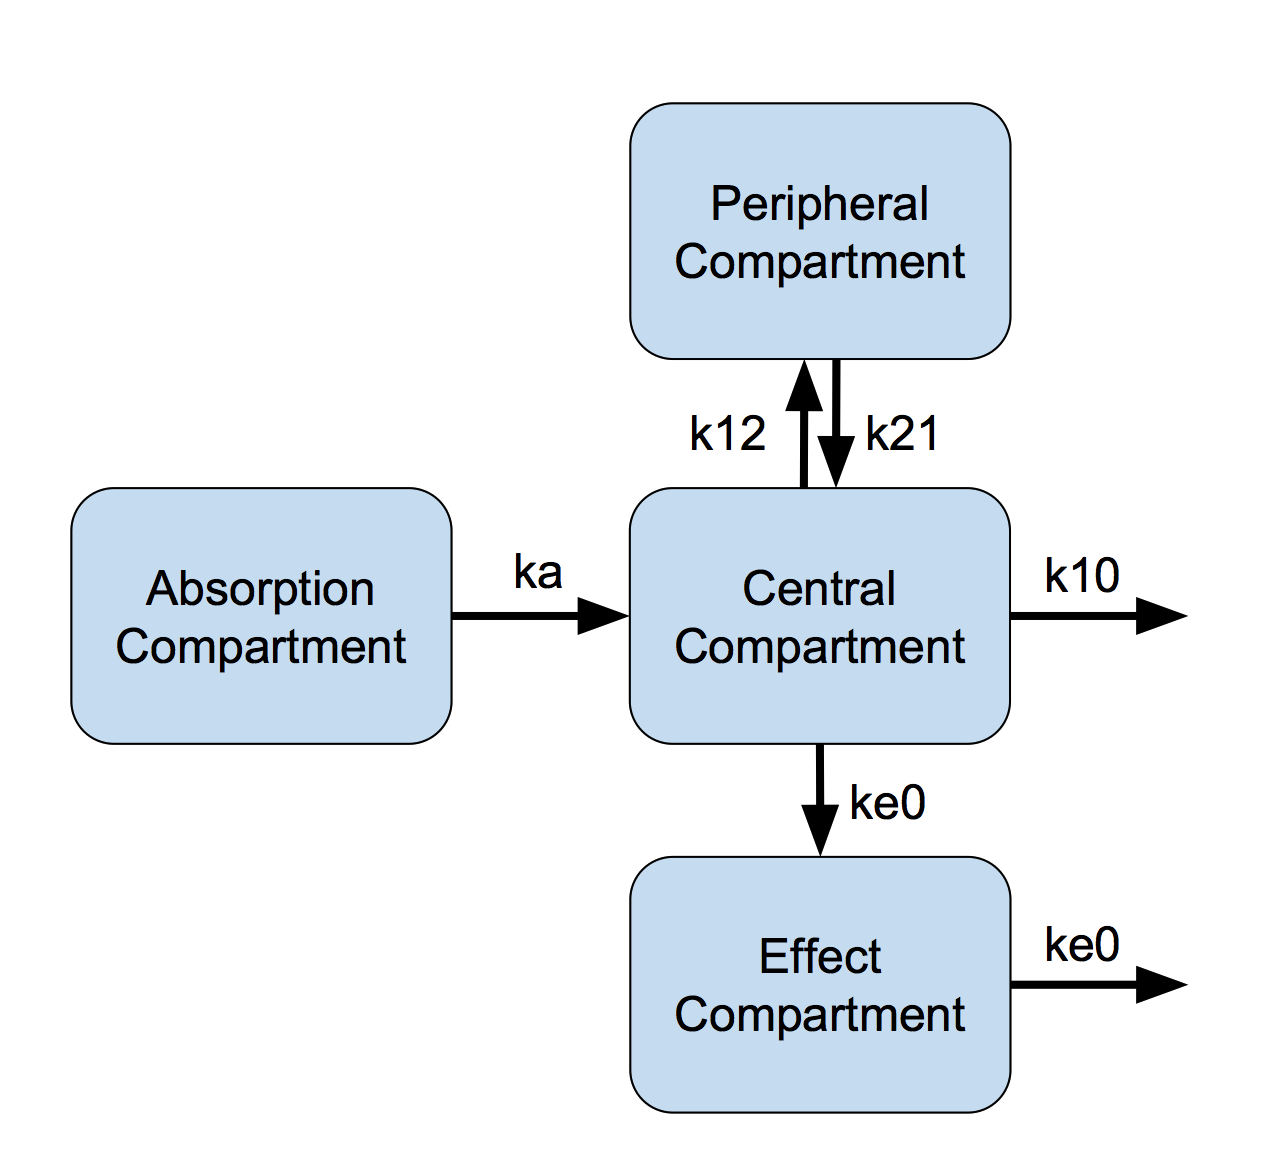
\includegraphics[width=3.5in,trim=0in 0in 0 0in]{graphics/effCptModel.png}
\caption{Effect Compartment Model}
\label{effCptModel}
\end{figure}

\subsubsection*{Effect Compartment Model for PD response ($R$)}
\begin{eqnarray*}
R_{ij} &\sim& N\left(\widehat{R}_{ij},\sigma_{R}^2\right) \\
\widehat{R}_{ij} &=& \frac{E_{max}c_{eij}}{EC_{50j} + c_{eij}} \\
c_{e\cdot j}^\prime &=& k_{e0j}\left(c_{\cdot j} - c_{e\cdot j}\right) \\
\log\left(EC_{50j}, k_{e0j}\right) &\sim& N\left(\log\left(\widehat{EC}_{50}, \widehat{k}_{e0}\right),\Omega_R\right) \\
\left(E_{max}, \widehat{EC}_{50},\widehat{k}_{e0}\right) &=& \left(100, 100.7, 1\right) \\
\Omega_R &=& \left(\begin{array}{cc} 0.2^2 & 0 \\ 0 & 0.25^2  \end{array}\right), \ \ \ \sigma_R = 10
\end{eqnarray*}

The PK and the PD data are simulated using the following treatment.
\begin{itemize}
  \item Phase I study
  \begin{itemize}
    \item Single dose and multiple doses
    \item Parallel dose escalation design
    \item 25 subjects per dose
    \item Single doses: 1.25, 5, 10, 20, and 40 mg 
    \item PK: plasma concentration of parent drug ($c$)
    \item PD response: Emax function of effect compartment concentration ($R$)
    \item PK and PD measured at 0.083, 0.167, 0.25, 0.5, 0.75, 1, 2, 3, 4, 6, 8, 12, 18, and 24 hours
  \end{itemize}
  \item Phase IIa trial in patients
  \begin{itemize}
    \item 100 subjects
    \item Multiple doses: 20 mg
    \item sparse PK and PD data (3-6 samples per patient)
  \end{itemize}
\end{itemize}

The model is simultaneously fitted to the PK and the PD data. For this effect compartment model, we construct a constant rate matrix and use \texttt{linOdeModel}. Correct use of Torsten requires the user pass the entire event history (observation and dosing events) for an individual to the function. Thus the Stan model shows the call to \texttt{linOdeModel} within a loop over the individual subjects rather than over the individual observations.

\begin{figure}
\caption{Stan language for fitting an effect compartment model using \texttt{linOdeModel} (abstract)}
\begin{tiny}
\begin{center}
\begin{fmpage}{\textwidth - .75in}
\begin{lstlisting}[basicstyle=\tiny\ttfamily,mathescape=true,flexiblecolumns=true,frame=single,escapeinside=`']
transformed parameters {
  for(j in 1:nSubjects){
                             $\vdots$
  Omega = quad_form_diag(rho, omega);

  for(j in 1:nSubjects){
    CL[j] = exp(logtheta[j, 1]) * (weight[j] / 70)^0.75;
    Q[j] = exp(logtheta[j, 2]) * (weight[j] / 70)^0.75;
    V1[j] = exp(logtheta[j, 3]) * weight[j] / 70;
    V2[j] = exp(logtheta[j, 4]) * weight[j] / 70;
    ka[j] = exp(logtheta[j, 5]);
    ke0[j] = exp(logKe0[j]);
    EC50[j] = exp(logEC50[j]);

    k10 = CL[j] / V1[j];
    k12 = Q[j] / V1[j];
    k21 = Q[j] / V2[j];

    K = rep_matrix(0, 4, 4);
    K[1, 1] = -ka[j];
    K[2, 1] = ka[j];
    K[2, 2] = -(k10 + k12);
    K[2, 3] = k21;
    K[3, 2] = k12;
    K[3, 3] = -k21;
    K[4, 2] = ke0[j];
    K[4, 4] = -ke0[j];
                        
    ke0[j] = exp(logKe0[j]);
    EC50[j] = exp(logEC50[j]);

    K = rep_matrix(0, 4, 4);
    
    K[1, 1] = -ka[j];
    K[2, 1] = ka[j];
    K[2, 2] = -(k10 + k12);
    K[2, 3] = k21;
    K[3, 2] = k12;
    K[3, 3] = -k21;
    K[4, 2] = ke0[j];
    K[4, 4] = -ke0[j];
           
    x[start[j]:end[j],] = `\textcolor{red}{linOdeModel}'(time[start[j]:end[j]], 
                                                 amt[start[j]:end[j]], rate[start[j]:end[j]],
                                                 ii[start[j]:end[j]], evid[start[j]:end[j]],
                                                 cmt[start[j]:end[j]], addl[start[j]:end[j]], 
                                                 ss[start[j]:end[j]], K, biovar, tlag);

    cHat[start[j]:end[j]] = 1000 * x[start[j]:end[j], 2] ./ V1[j];
    ceHat[start[j]:end[j]] = 1000 * x[start[j]:end[j], 4] ./ V1[j];
    respHat[start[j]:end[j]] = 100 * ceHat[start[j]:end[j]] ./ 
       (EC50[j] + ceHat[start[j]:end[j]]);
  }

  for(i in 1:nObs){
    cHatObs[i] = cHat[iObs[i]];
    respHatObs[i] = respHat[iObs[i]];
  }
}
                             $\vdots$  
} 
\end{lstlisting}
\end{fmpage}
\end{center}
\end{tiny} 
\label{effCptModelCode}
\end{figure}

\subsubsection*{Results} We use the same diagnosis tools as for the previous example. The MCMC history plots (figure \ref{effCptModelMCMC}) suggest the 4 chains have converged to common distributions. We note some minor auto-correlations for $lp\_$ (the log posterior) and for IIV parameters: specifically $\Omega_{ke\_0}$ and $\rho$. The correlation matrix $\rho$ does not explicitly appear in the model, but it is used to construct $\Omega$, which parametrizes the PK IIV. The fits to the plasma concentration  (figure~\ref{effCptModelPredictionsPK}) are in close agreement with the data, notably for the sparse data case (phase IIa study). The fits to the PD data (figure~\ref{effCptModelPredictionsPD}) look good, though the data is more noisy. The model reflects the noise by producing larger credible intervals. The estimated values of the parameters are consistent with the values used to simulate the data.

\begin{table}[!htb]
\centering
\caption{Summary of the MCMC simulations of the marginal posterior distributions of the model parameters for example 2}
\begin{tabular}{rrrrrrrrrrr}
  \hline
 & mean & se\_mean & sd & 2.5\% & 25\% & 50\% & 75\% & 97.5\% & n\_eff & Rhat \\ 
  \hline
CLHat & 10.095 & 0.003 & 0.201 & 9.712 & 9.958 & 10.096 & 10.231 & 10.483 & 4000.000 & 0.999 \\
QHat & 14.867 & 0.014 & 0.357 & 14.182 & 14.620 & 14.862 & 15.106 & 15.563 & 678.208 & 1.007 \\
V1Hat & 34.188 & 0.067 & 1.089 & 31.940 & 33.494 & 34.214 & 34.918 & 36.251 & 267.748 & 1.016 \\
V2Hat & 103.562 & 0.076 & 2.925 & 98.031 & 101.600 & 103.455 & 105.472 & 109.583 & 488.296 & 1.001 \\
kaHat & 1.930 & 0.004 & 0.077 & 1.771 & 1.880 & 1.933 & 1.982 & 2.076 & 334.888 & 1.014 \\
ke0Hat & 1.050 & 0.001 & 0.044 & 0.967 & 1.020 & 1.051 & 1.078 & 1.137 & 164.741 & 1.000 \\
EC50Hat & 104.337 & 0.040 & 2.100 & 100.169 & 102.909 & 104.345 & 105.768 & 108.351 & 744.041 & 1.000 \\
sigma & 0.099 & 0.000 & 0.002 & 0.095 & 0.097 & 0.099 & 0.100 & 0.103 & 906.342 & 1.002 \\
sigmaResp & 10.156 & 0.003 & 0.197 & 9.779 & 10.023 & 10.154 & 10.286 & 10.552 & 4000.000 & 1.000 \\
omega[1] & 0.270 & 0.000 & 0.016 & 0.241 & 0.259 & 0.269 & 0.280 & 0.302 & 4000.000 & 1.001 \\
omega[2] & 0.231 & 0.001 & 0.021 & 0.192 & 0.217 & 0.230 & 0.245 & 0.275 & 531.512 & 1.006 \\
omega[3] & 0.219 & 0.002 & 0.031 & 0.158 & 0.199 & 0.218 & 0.238 & 0.281 & 158.198 & 1.017 \\
omega[4] & 0.267 & 0.001 & 0.026 & 0.218 & 0.249 & 0.266 & 0.284 & 0.319 & 684.870 & 1.001 \\
omega[5] & 0.285 & 0.002 & 0.037 & 0.214 & 0.259 & 0.284 & 0.309 & 0.361 & 284.545 & 1.009 \\
omegaKe0 & 0.271 & 0.003 & 0.047 & 0.183 & 0.239 & 0.271 & 0.303 & 0.363 & 217.350 & 1.007 \\
omegaEC50 & 0.213 & 0.001 & 0.021 & 0.174 & 0.199 & 0.213 & 0.227 & 0.255 & 190.193 & 1.000 \\
  \hline
\end{tabular}
\end{table}

\clearpage

\begin{figure}[!htb]
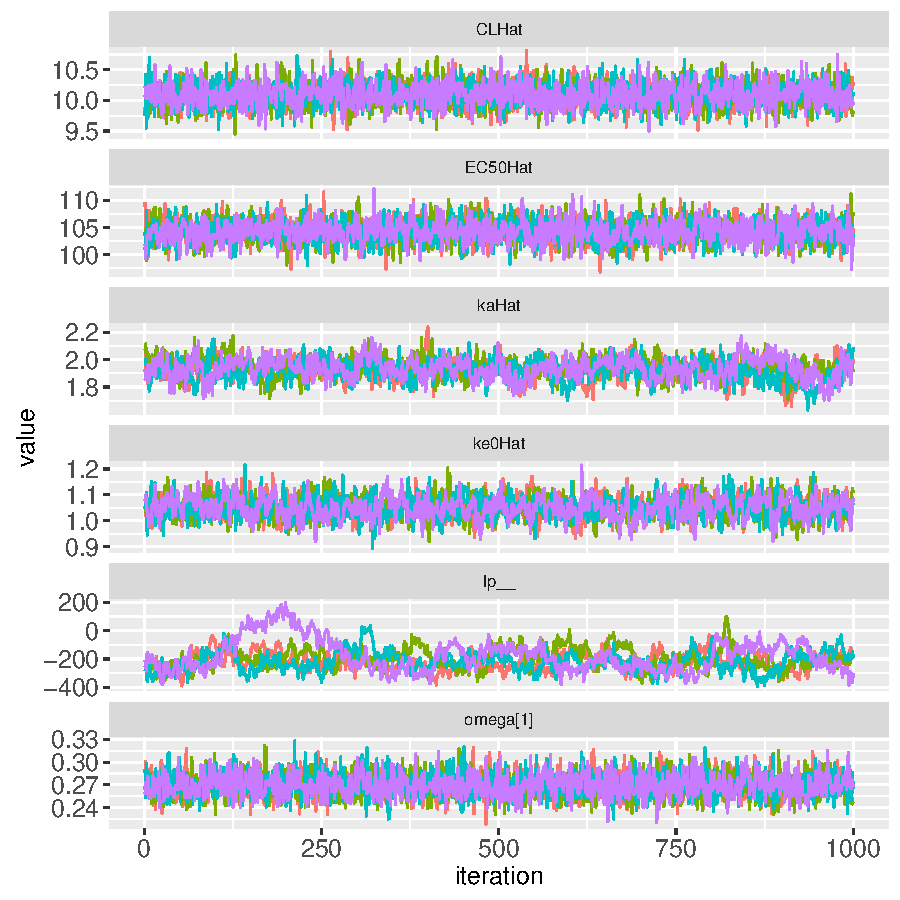
\includegraphics[width=3.0in,trim=0in 0in 0 0in]{graphics/effCptModelTorsten/effCptModelTorstenPlots001.pdf}
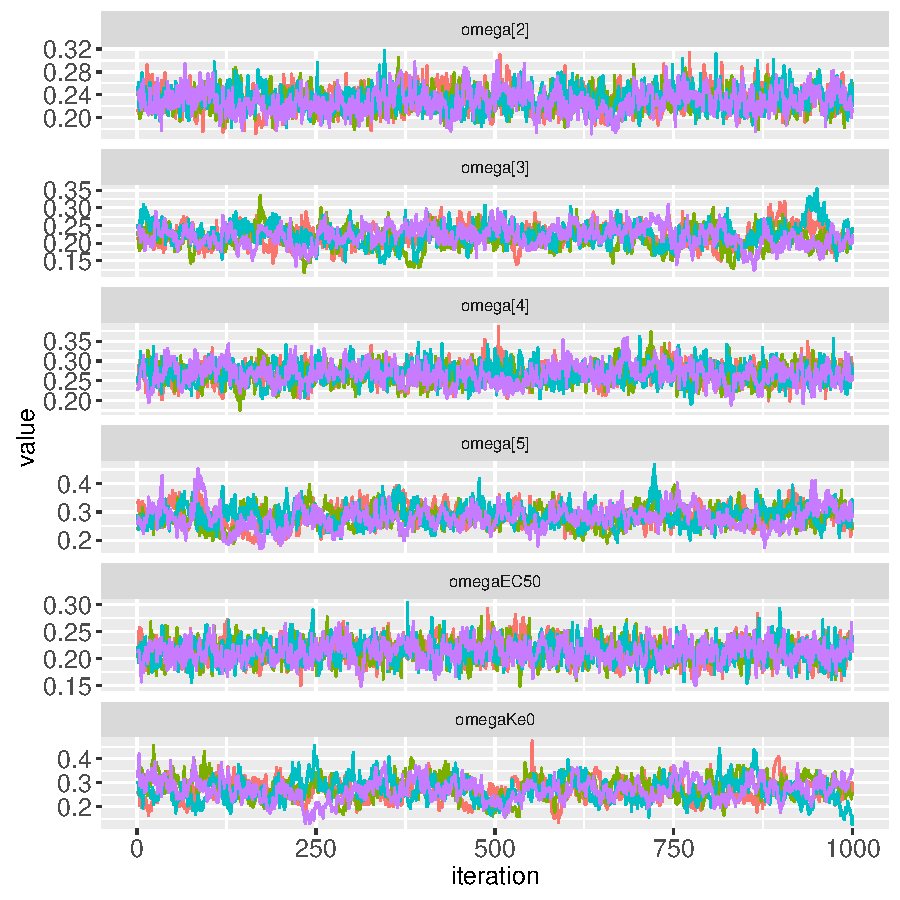
\includegraphics[width=3.0in,trim=0in 0in 0 0in]{graphics/effCptModelTorsten/effCptModelTorstenPlots002.pdf}
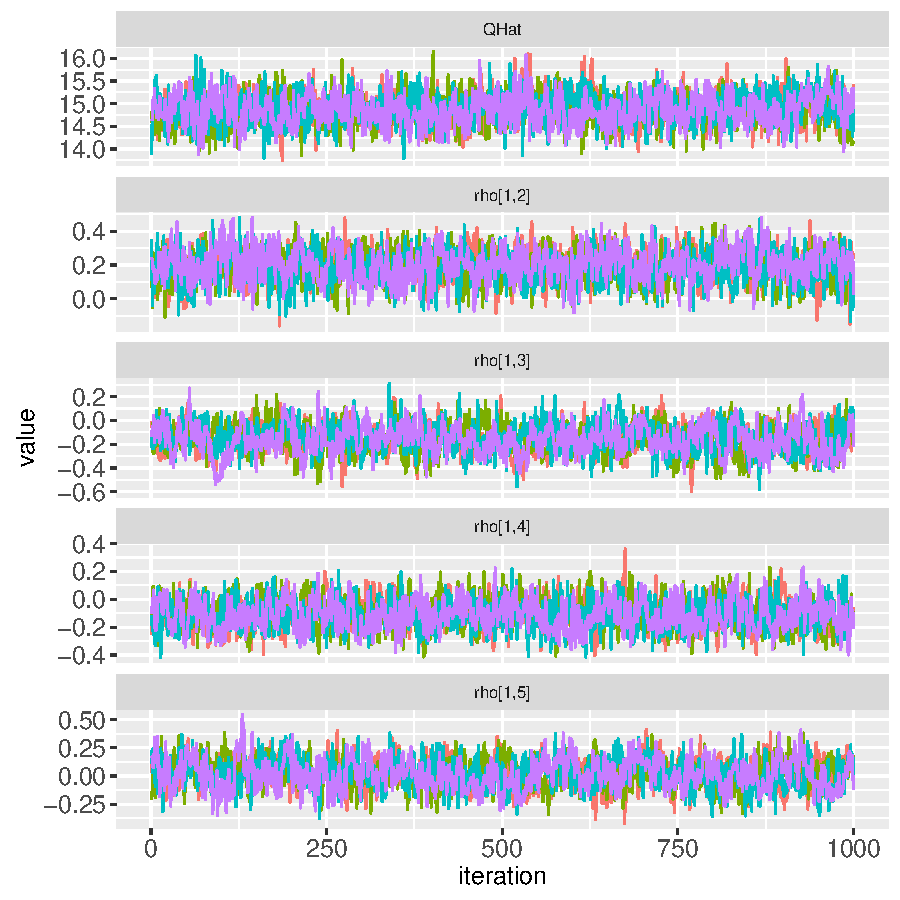
\includegraphics[width=3.0in,trim=0in 0in 0 0in]{graphics/effCptModelTorsten/effCptModelTorstenPlots003.pdf}
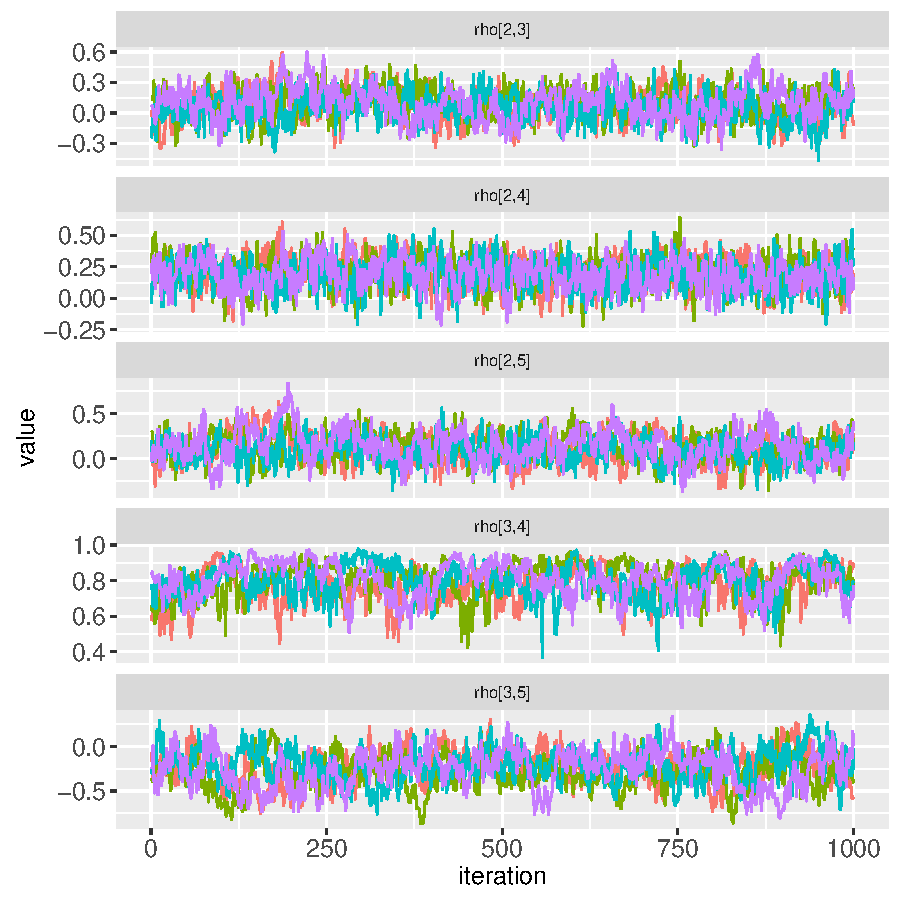
\includegraphics[width=3.0in,trim=0in 0in 0 0in]{graphics/effCptModelTorsten/effCptModelTorstenPlots004.pdf}
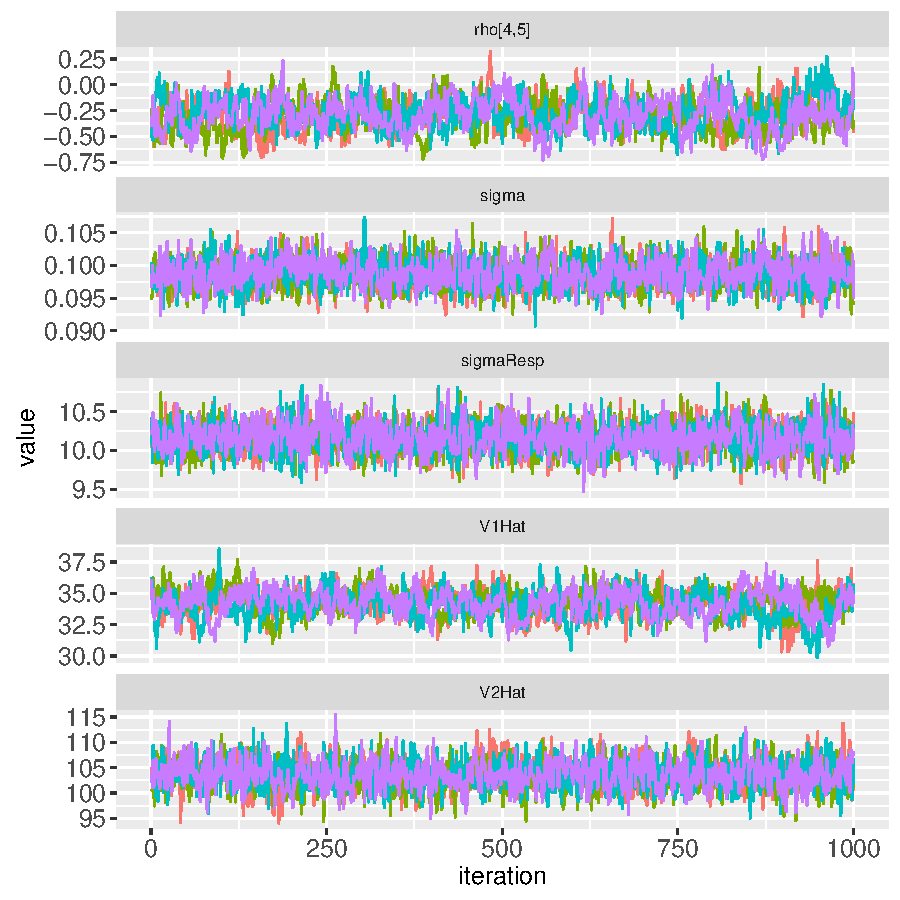
\includegraphics[width=3.0in,trim=0in 0in 0 0in]{graphics/effCptModelTorsten/effCptModelTorstenPlots005.pdf}
\caption{{MCMC history plots for the parameters of an Effect Compartment Model (each color corresponds to a different chain) for example 2}}
\label{effCptModelMCMC}
\end{figure}

\begin{figure}[!htb]
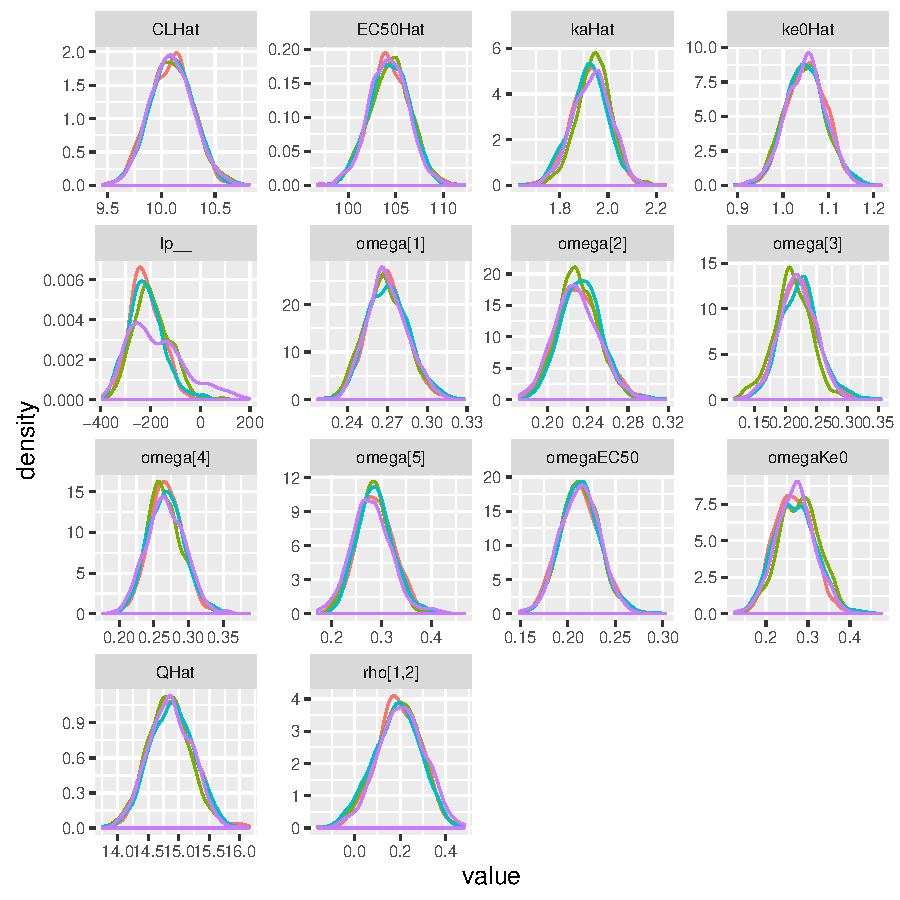
\includegraphics[width=3.0in,trim=0in 0in 0 0in]{graphics/effCptModelTorsten/effCptModelTorstenPlots006.pdf}
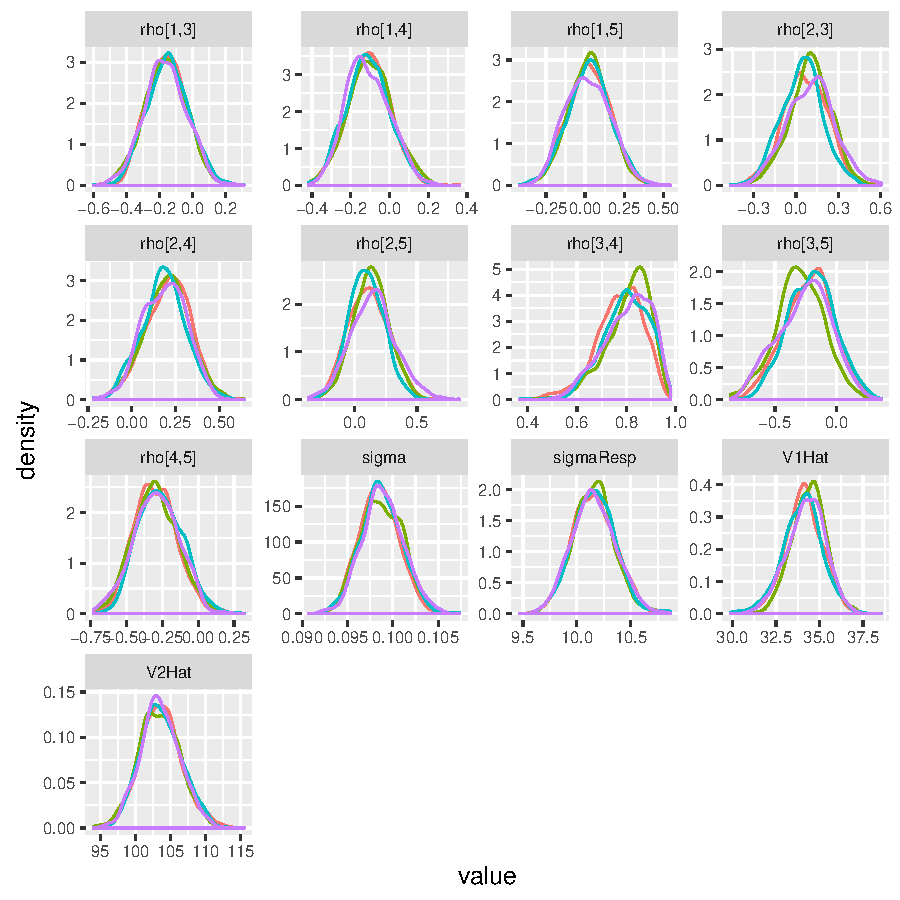
\includegraphics[width=3.0in,trim=0in 0in 0 0in]{graphics/effCptModelTorsten/effCptModelTorstenPlots007.pdf}
\caption{{Posterior Marginal Densities of the Model Parameters of an Effect Compartment Model (each color corresponds to a different chain) for example 2}}
\label{effCptModelDens}
\end{figure}

\begin{figure}[htbp]
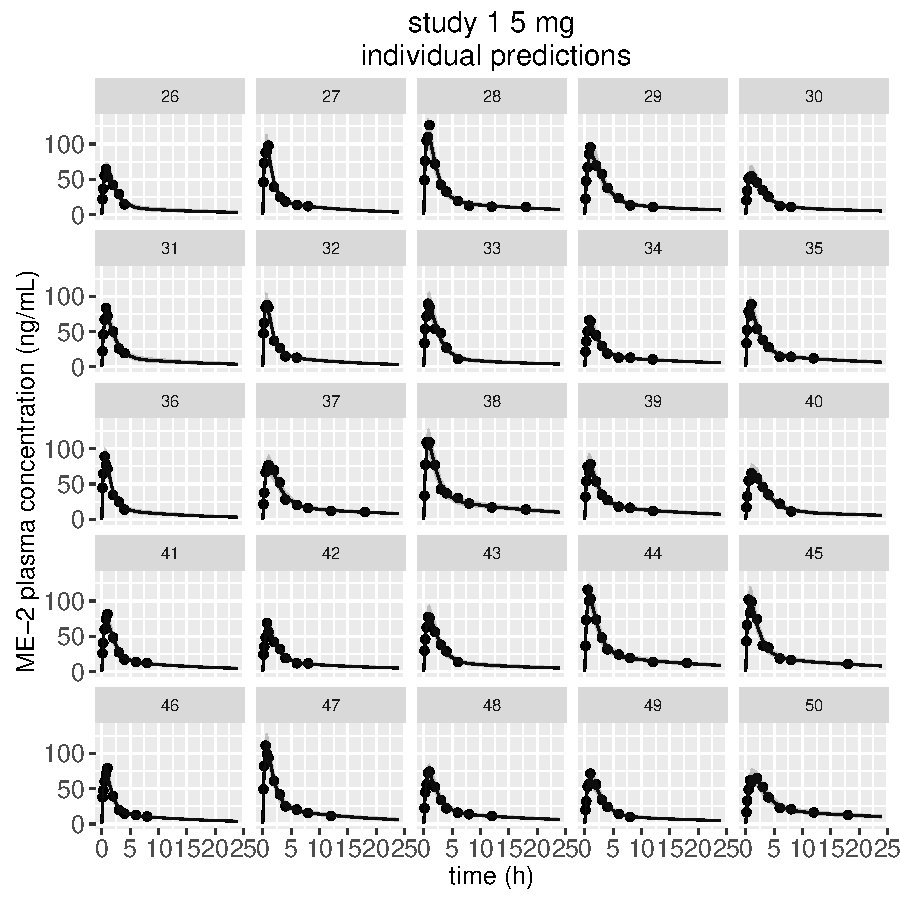
\includegraphics[width=1.5in,trim=0in 0in 0 0in]{graphics/effCptModelTorsten/effCptModelTorstenPlots011.pdf}
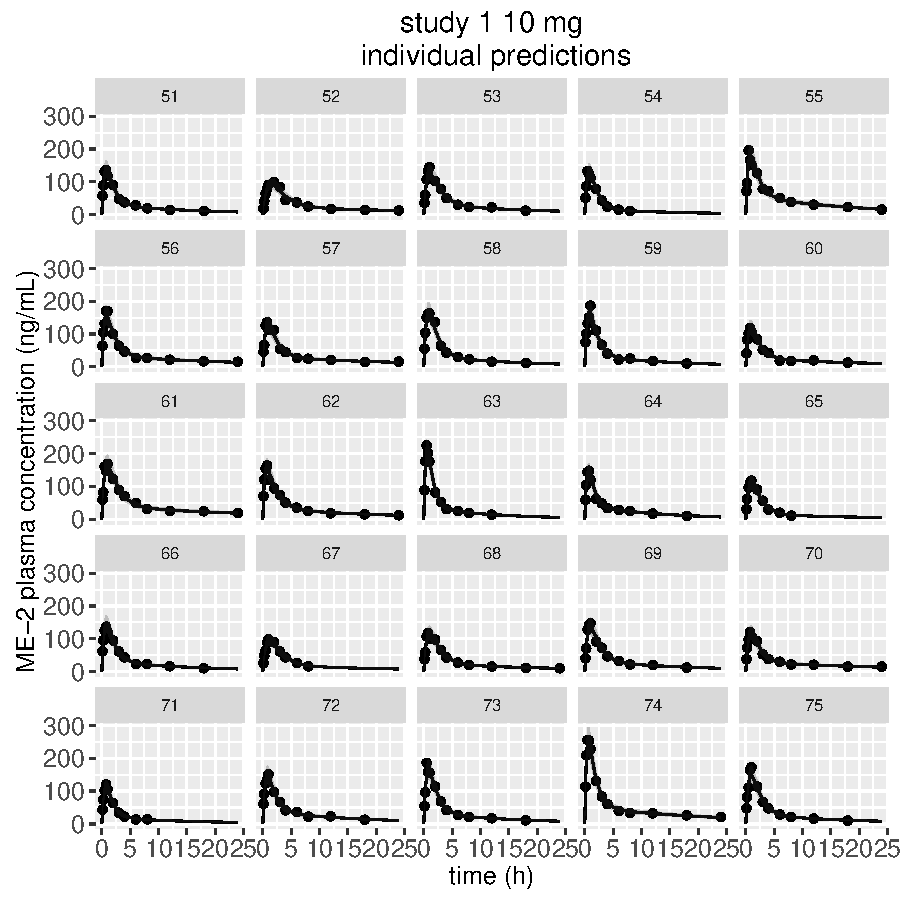
\includegraphics[width=1.5in,trim=0in 0in 0 0in]{graphics/effCptModelTorsten/effCptModelTorstenPlots012.pdf}
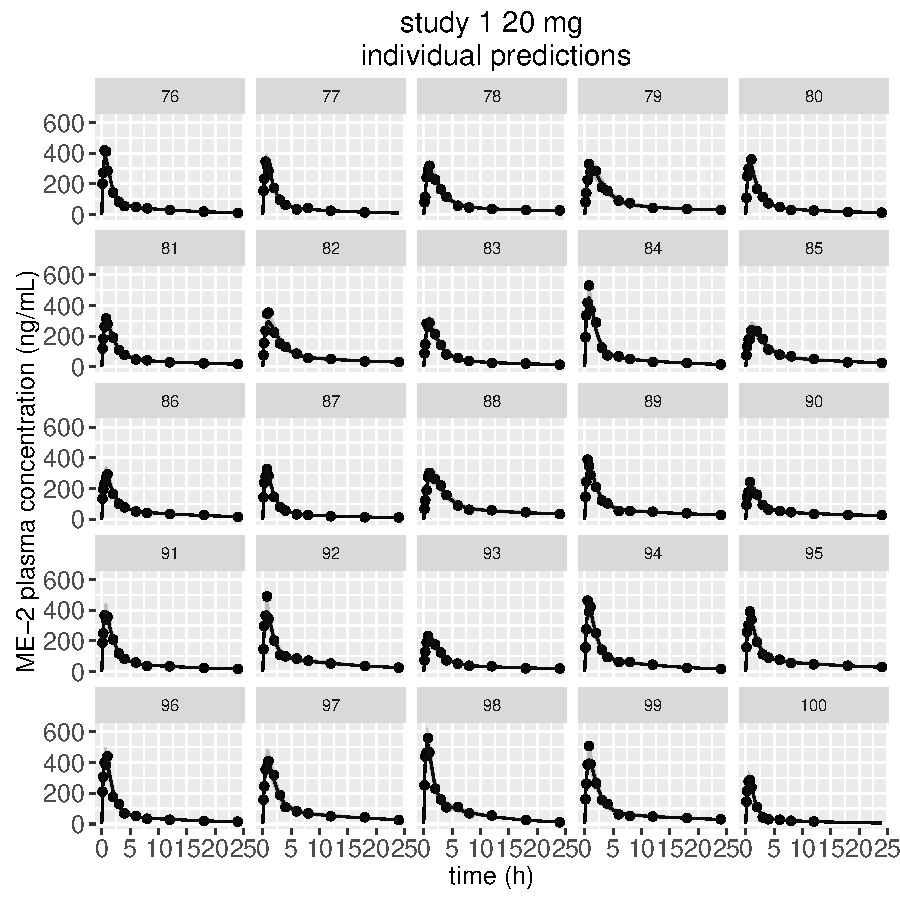
\includegraphics[width=1.5in,trim=0in 0in 0 0in]{graphics/effCptModelTorsten/effCptModelTorstenPlots013.pdf}
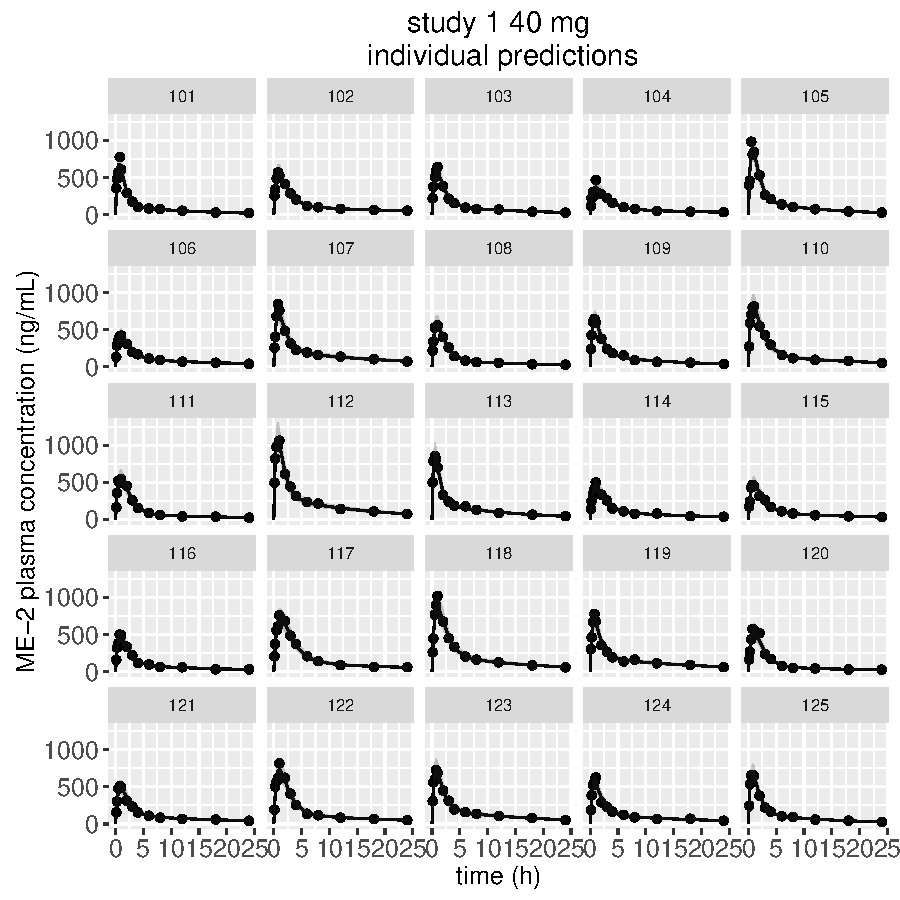
\includegraphics[width=1.5in,trim=0in 0in 0 0in]{graphics/effCptModelTorsten/effCptModelTorstenPlots014.pdf}
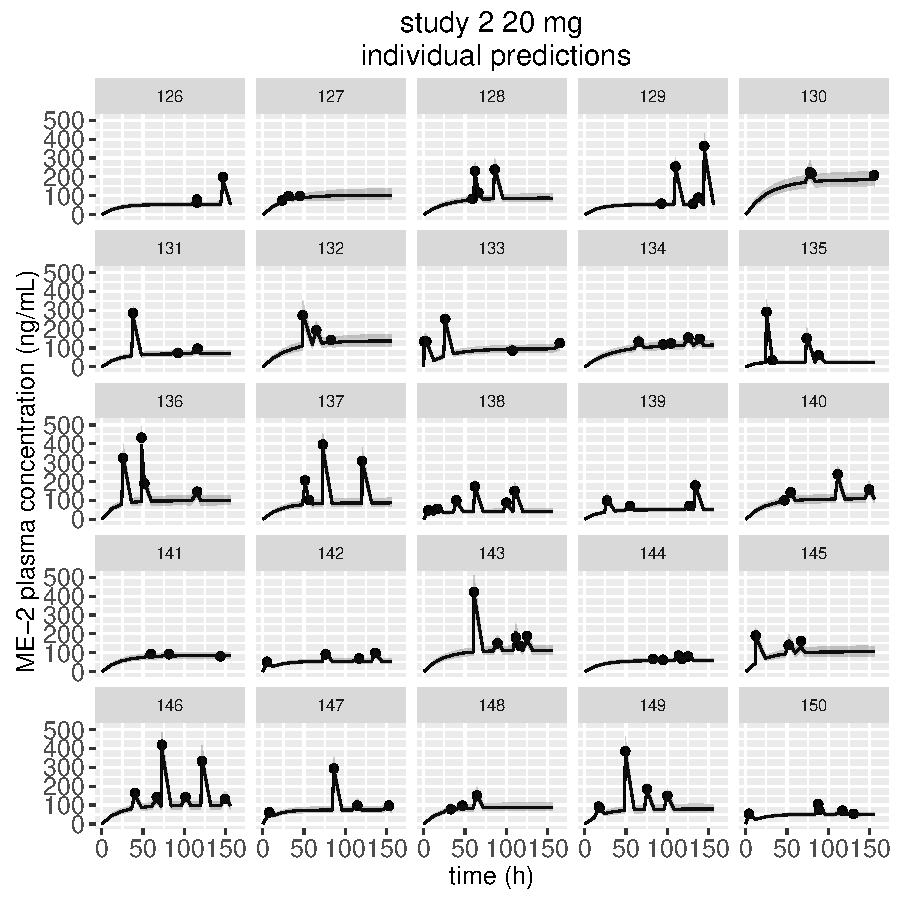
\includegraphics[width=1.5in,trim=0in 0in 0 0in]{graphics/effCptModelTorsten/effCptModelTorstenPlots015.pdf}
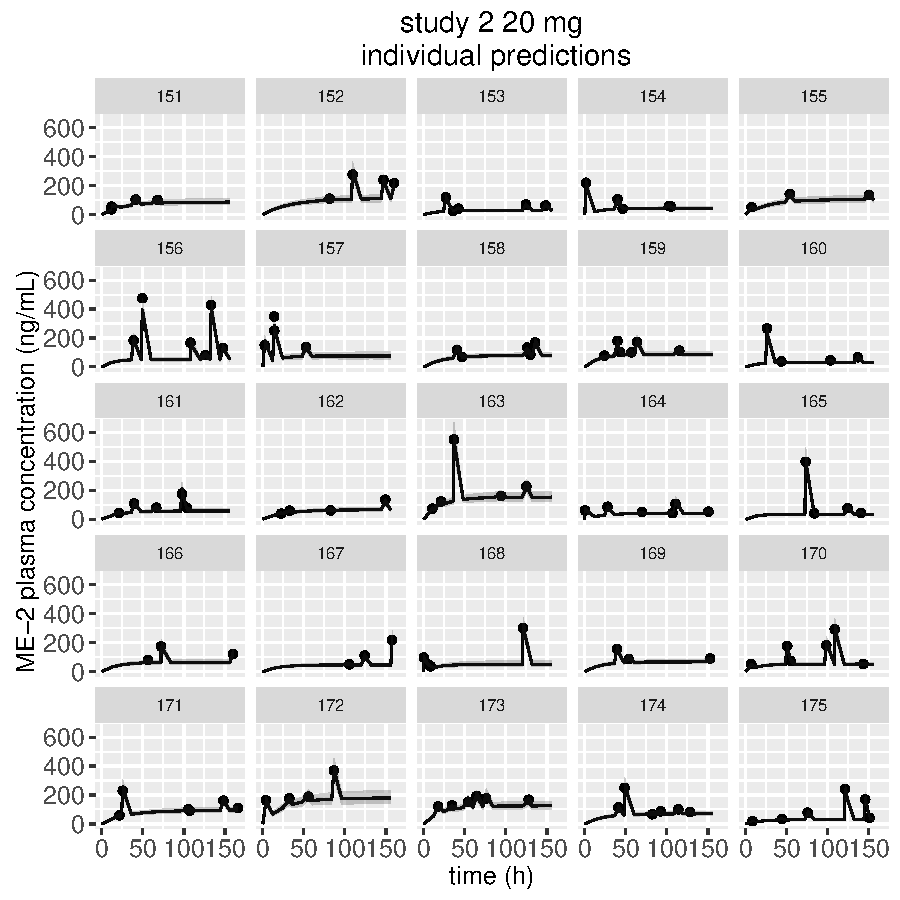
\includegraphics[width=1.5in,trim=0in 0in 0 0in]{graphics/effCptModelTorsten/effCptModelTorstenPlots016.pdf}
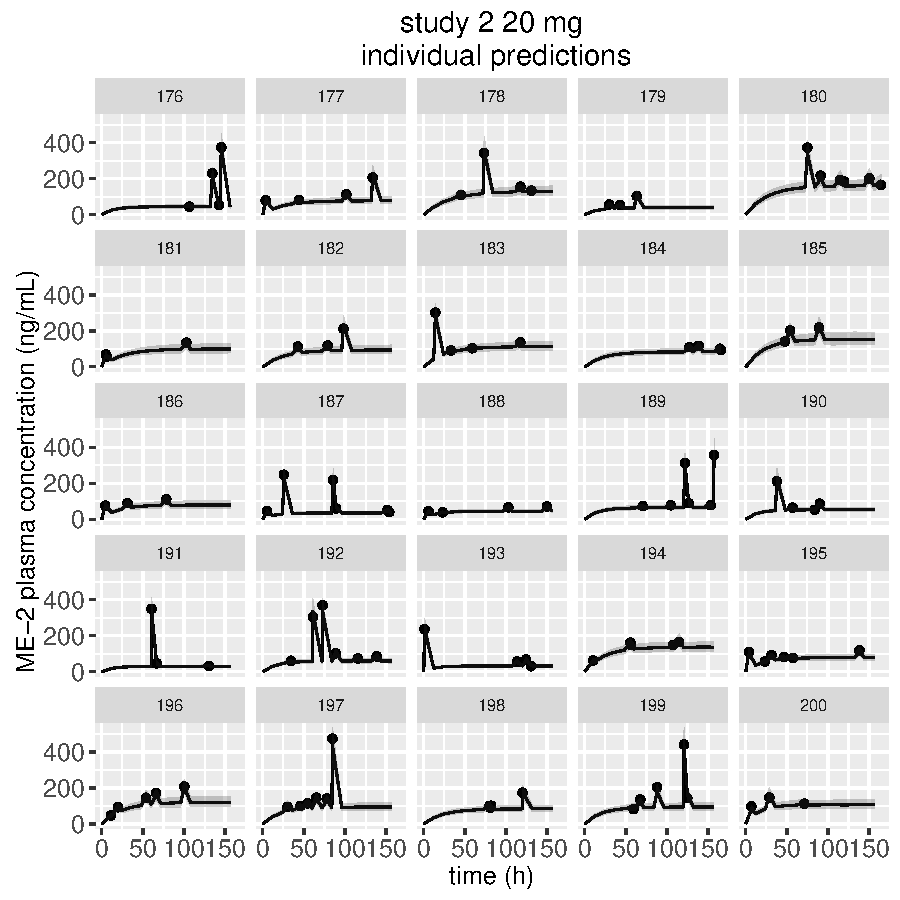
\includegraphics[width=1.5in,trim=0in 0in 0 0in]{graphics/effCptModelTorsten/effCptModelTorstenPlots017.pdf}
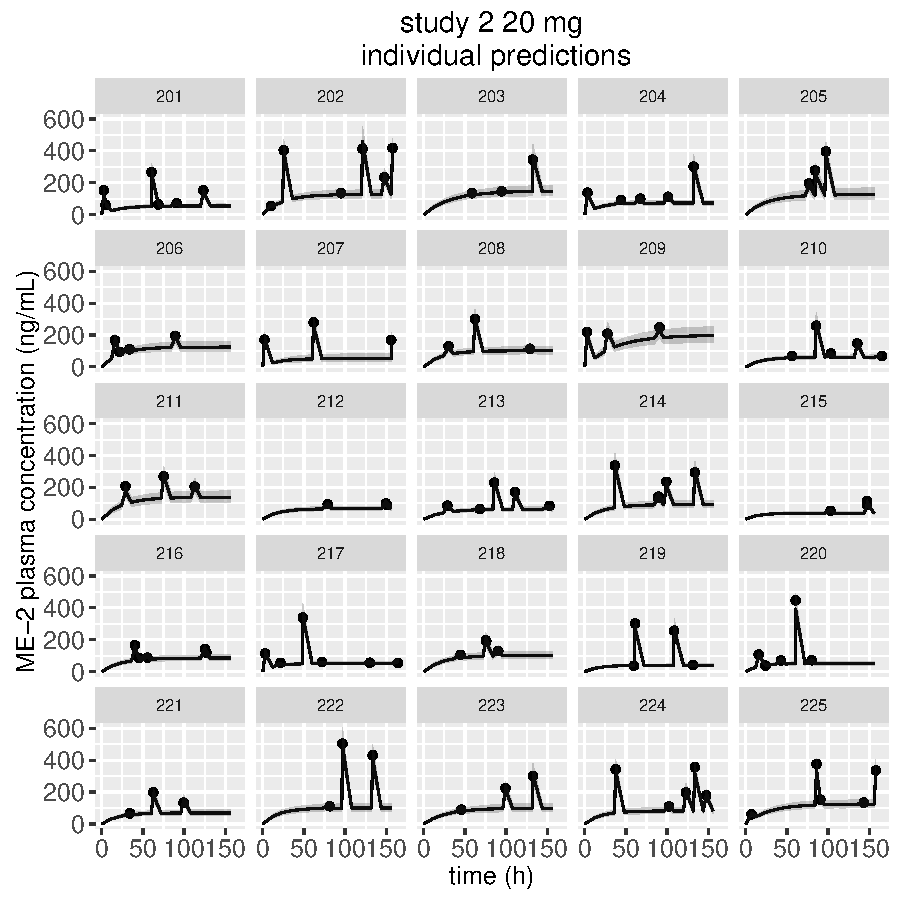
\includegraphics[width=1.5in,trim=0in 0in 0 0in]{graphics/effCptModelTorsten/effCptModelTorstenPlots018.pdf}
\caption{{Predicted (posterior median and 90 \% credible intervals) and observed plasma drug concentrations for example 2 for an Effect Compartment Model}}
\label{effCptModelPredictionsPK}
\end{figure}

\begin{figure}[htbp]
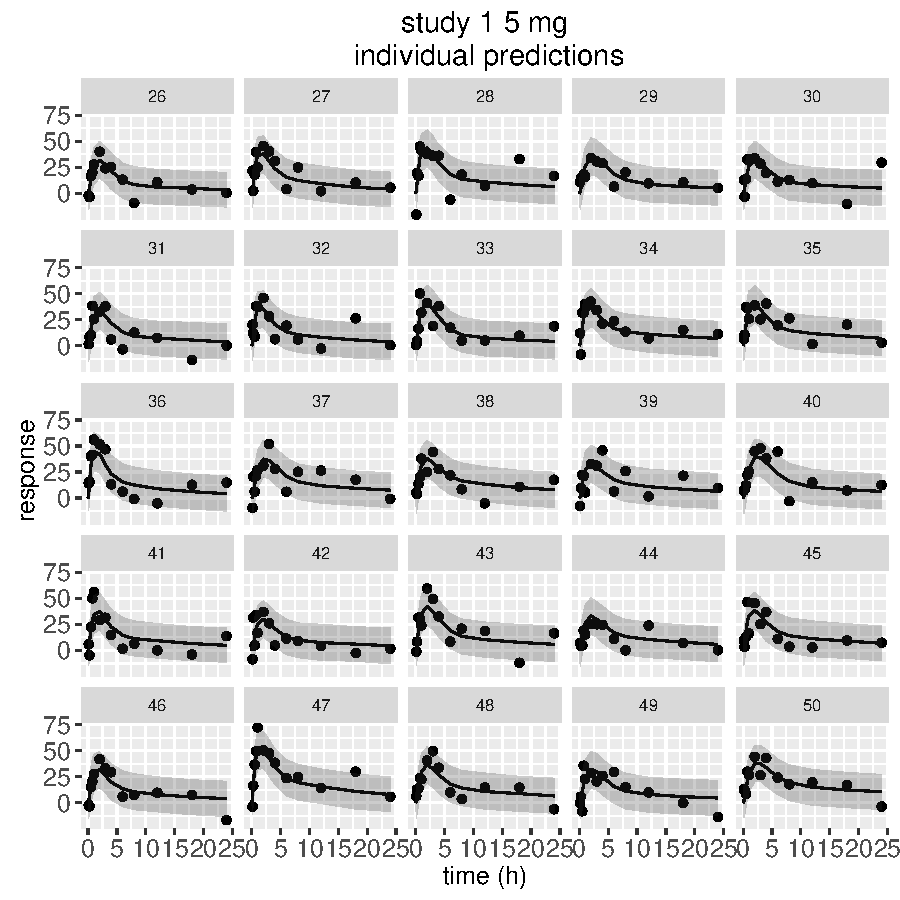
\includegraphics[width=1.5in,trim=0in 0in 0 0in]{graphics/effCptModelTorsten/effCptModelTorstenPlots019.pdf}
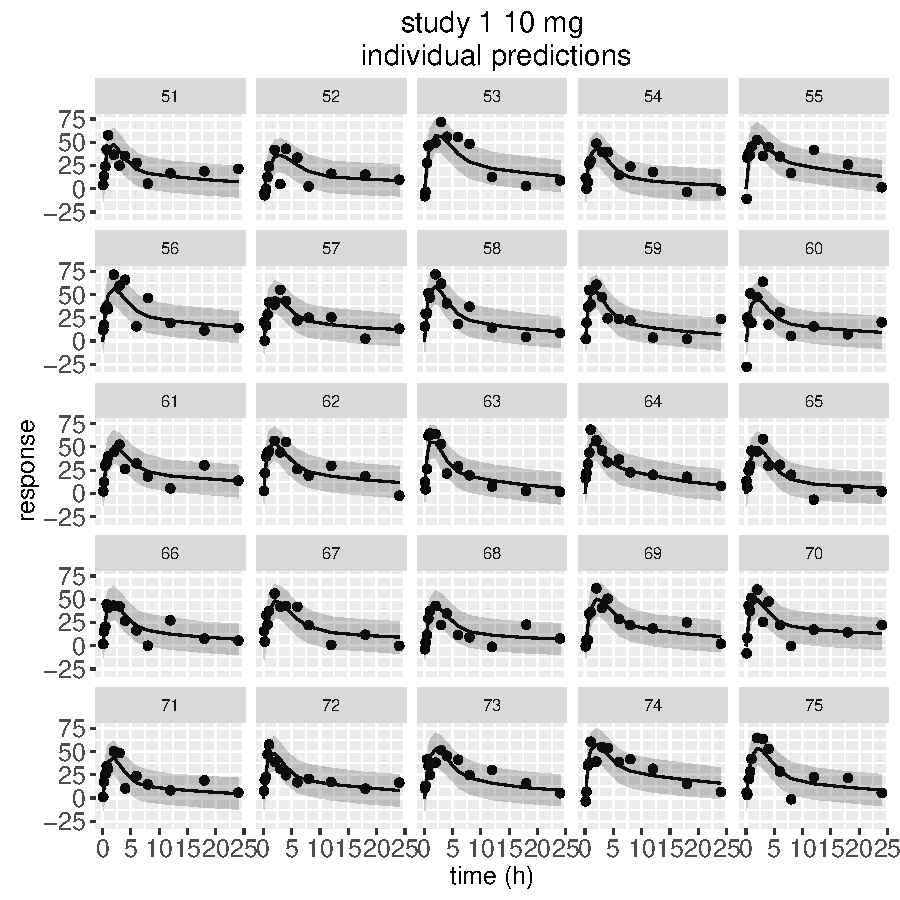
\includegraphics[width=1.5in,trim=0in 0in 0 0in]{graphics/effCptModelTorsten/effCptModelTorstenPlots020.pdf}
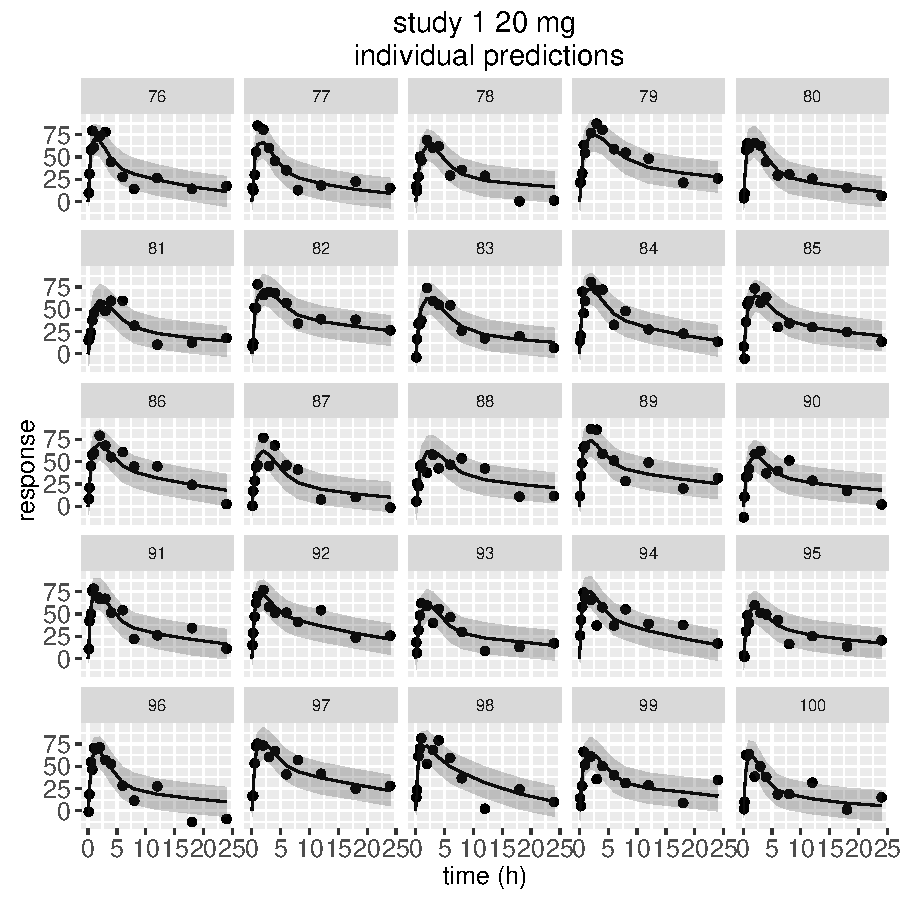
\includegraphics[width=1.5in,trim=0in 0in 0 0in]{graphics/effCptModelTorsten/effCptModelTorstenPlots021.pdf}
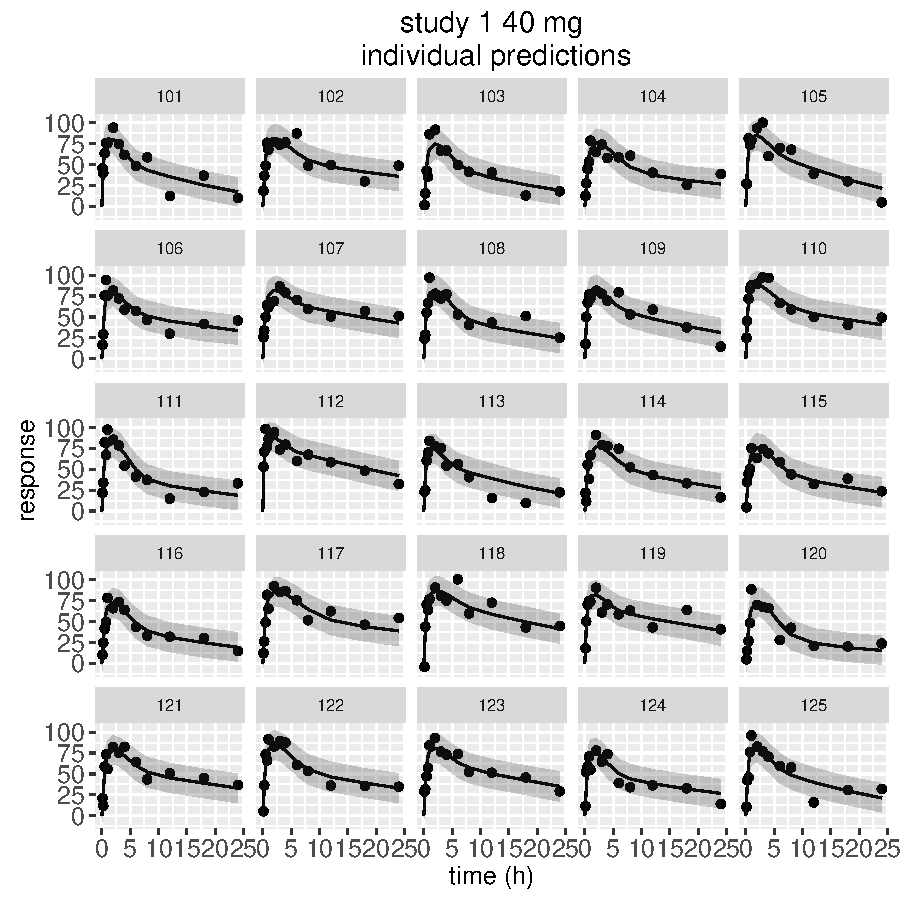
\includegraphics[width=1.5in,trim=0in 0in 0 0in]{graphics/effCptModelTorsten/effCptModelTorstenPlots022.pdf}
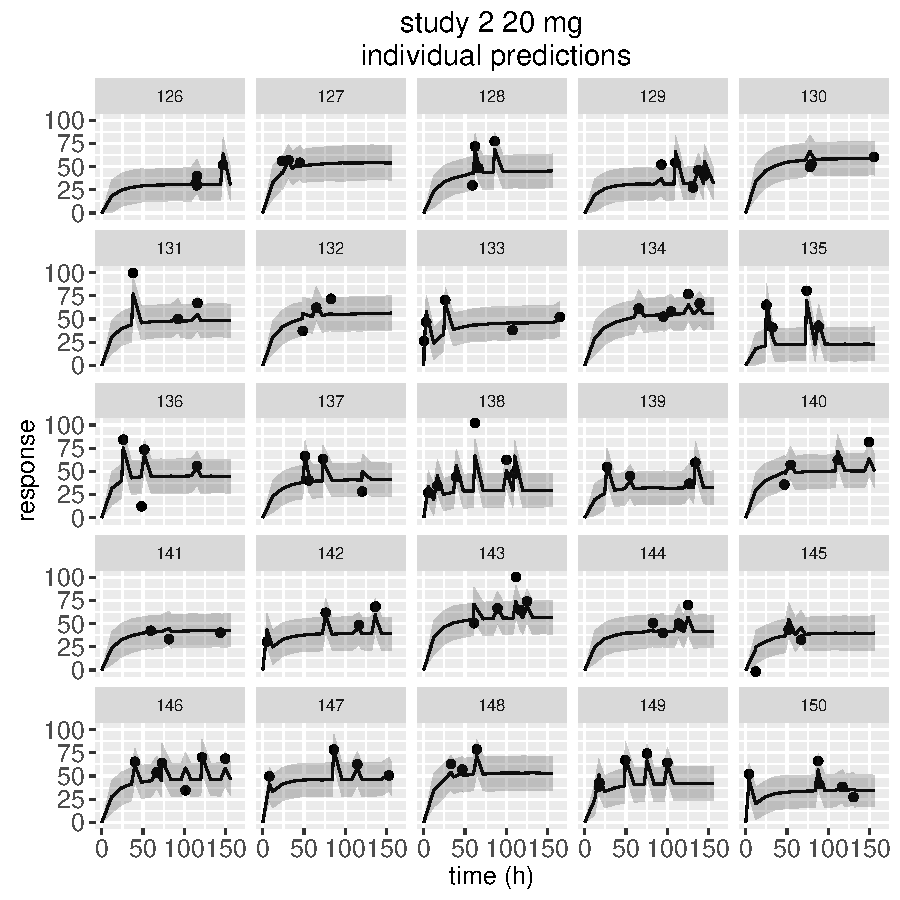
\includegraphics[width=1.5in,trim=0in 0in 0 0in]{graphics/effCptModelTorsten/effCptModelTorstenPlots023.pdf}
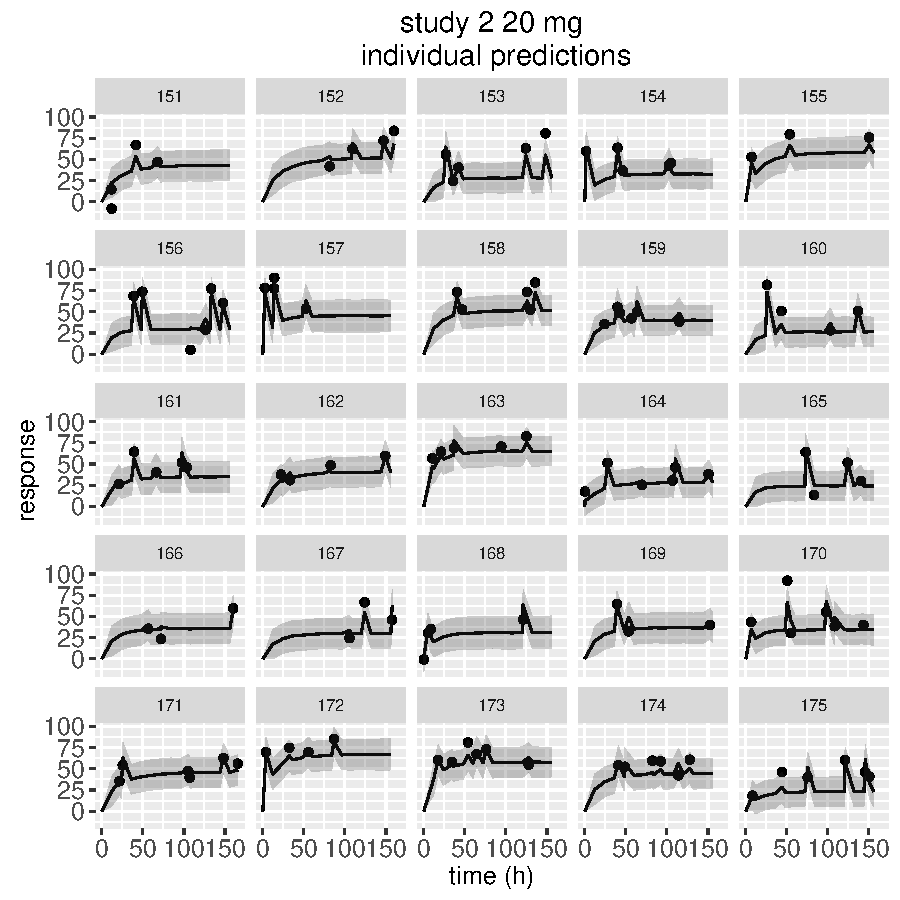
\includegraphics[width=1.5in,trim=0in 0in 0 0in]{graphics/effCptModelTorsten/effCptModelTorstenPlots024.pdf}
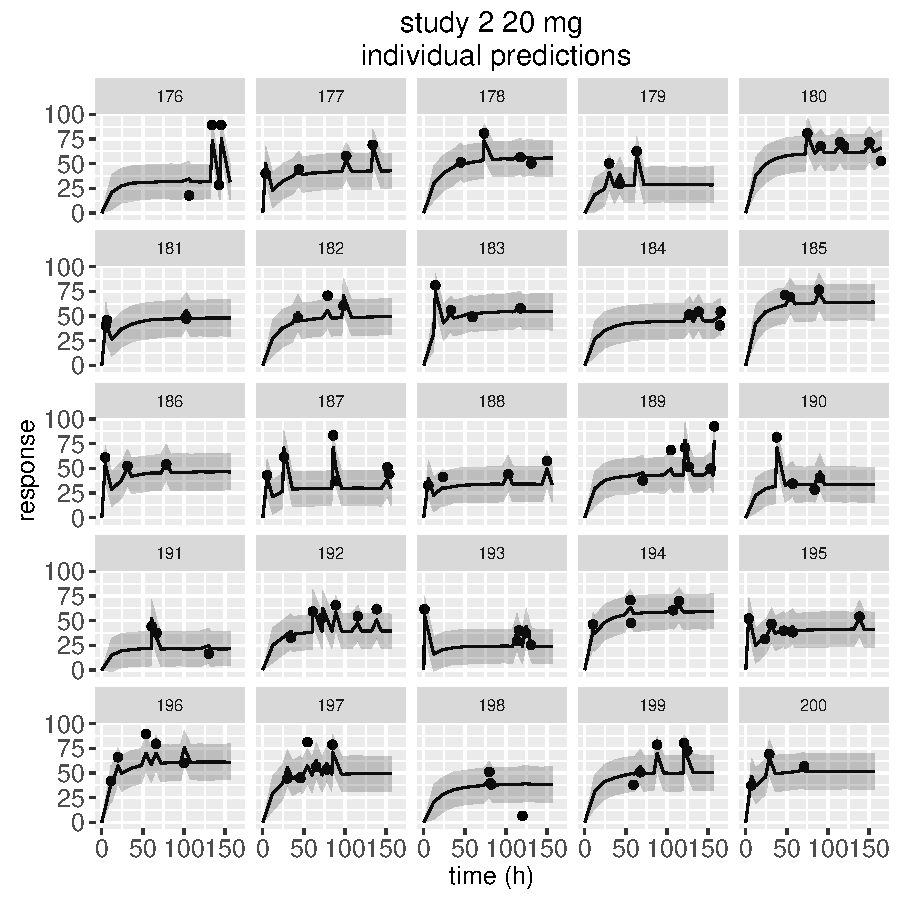
\includegraphics[width=1.5in,trim=0in 0in 0 0in]{graphics/effCptModelTorsten/effCptModelTorstenPlots025.pdf}
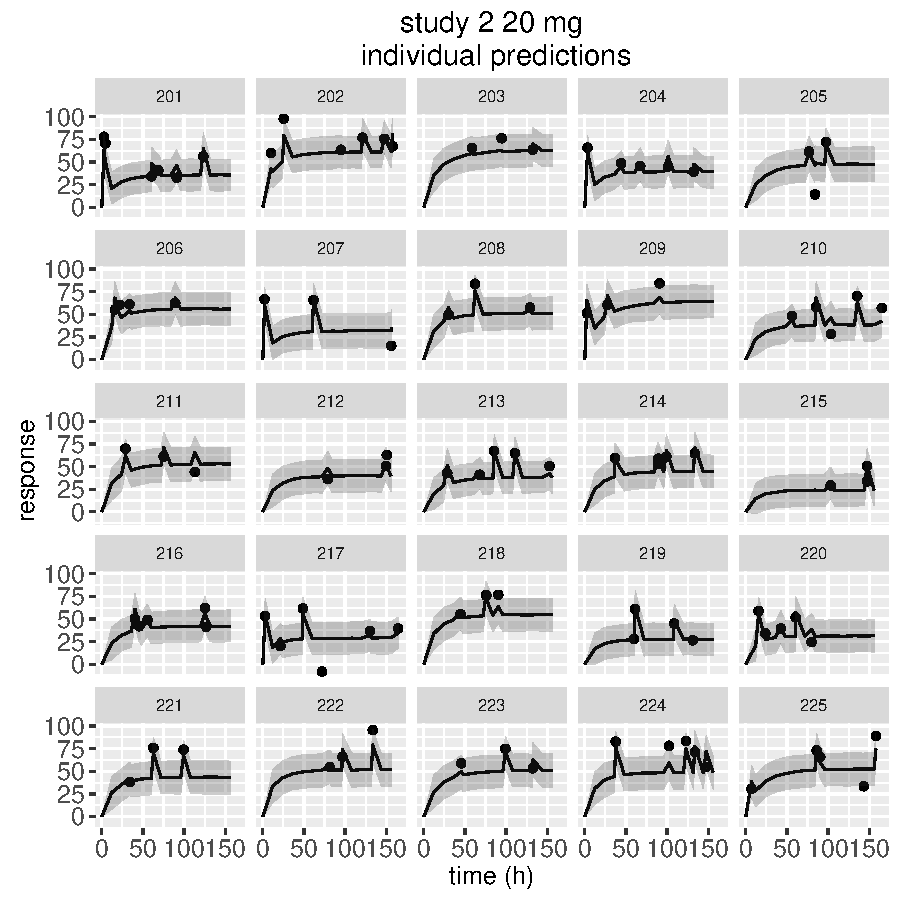
\includegraphics[width=1.5in,trim=0in 0in 0 0in]{graphics/effCptModelTorsten/effCptModelTorstenPlots026.pdf}
\caption{{Predicted (posterior median and 90 \% credible intervals) and observed PD Response for example 2}}
\label{effCptModelPredictionsPD}
\end{figure}

\clearpage

\subsection{Friberg-Karlsson Semi-Mechanistic Model \cite{2364}} \ \\ 

In this third example, we deal with a more sophisticated PD effect, described by a system of nonlinear ODEs. The PK effects are still described by a two compartment model with a first-order absorption. 

Neutropenia is observed in patients receiving an ME-2 drug. Our goal is to model the relation between neutrophil counts and drug exposure. Using a feedback mechanism, the body maintains the number of neutrophils at a baseline value (figure~\ref{FK}). While in the patient's blood, the drug impedes the production of neutrophils. As a result, the neutrophil count goes down, and after  the drug clears out, the feedback mechanism kicks in and brings the neutrophil count back to baseline.

{\bf Friberg-Karlsson Model for drug-induced myelosuppression ($ANC$)}

\begin{eqnarray*}
\log(ANC_{ij}) &\sim& N(Circ_{ij}, \sigma^2_{ANC}) \\
\log\left(MTT_j, Circ_{0j}, \alpha_j\right) &\sim& N\left(\log\left(\widehat{MTT}, \widehat{Circ_0}, \widehat{\alpha}\right), \Omega_{ANC}\right) \\
\left(\widehat{MTT}, \widehat{Circ}_0,\widehat{\alpha}, \gamma \right) &=& \left(125, 5, 2, 0.17\right) \\
\Omega_{ANC} &=& \left(\begin{array}{ccc} 0.2^2 & 0 & 0 \\ 0 & 0.35^2 & 0 \\ 0 & 0 & 0.2^2 \end{array}\right), \ \ \ \sigma_{ANC} = 0.1 \\
\Omega_{PK} &=& \left(\begin{array}{ccccc} 0.25^2 & 0 &a 0 & 0 & 0 \\ 0 & 0.4^2 & 0 & 0 & 0 \\
0 & 0 & 0.25^2 & 0 & 0 \\ 0 & 0 & 0 & 0.4^2 & 0 \\ 0 & 0 & 0 & 0 & 0.25^2  \end{array}\right)
\end{eqnarray*}

\begin{figure}[htbp]
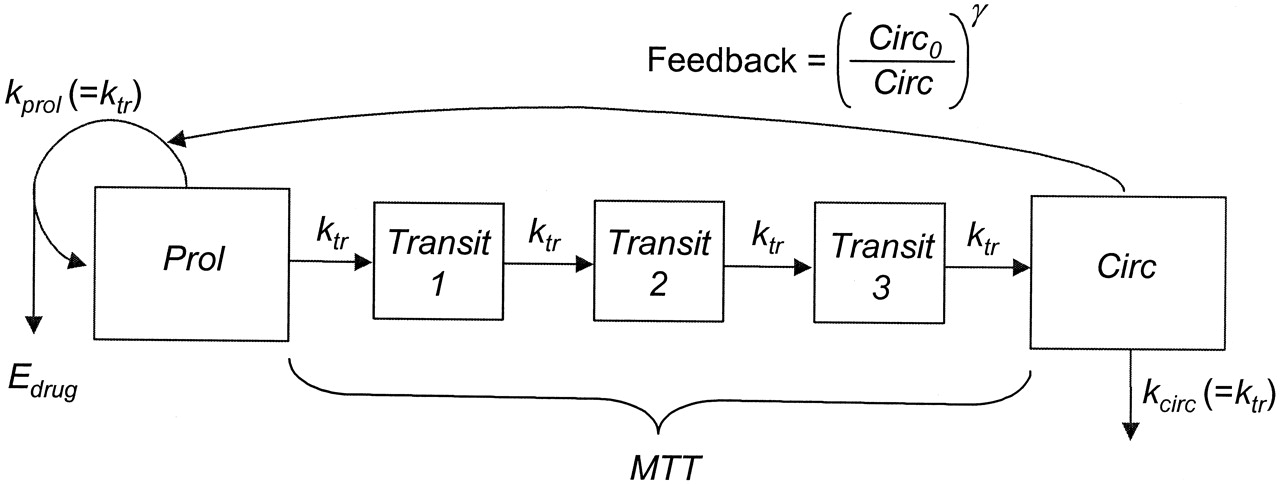
\includegraphics[width=3.5in,trim=0in 0in 0 0in]{graphics/neutrophilModel.jpg}
\caption{Friberg-Karlsson semi-mechanistic Model \cite{2364}}
\label{FK}
\end{figure}

The PK and the PD data are simulated using the following treatment.
\begin{itemize}
  \item Phase IIa trial in patients
  \begin{itemize}
    \item Multiple doses: 80,000 mg
    \item Parallel dose escalation design
    \item 15 subjects
    \item PK: plasma concentration of parent drug ($c$)
    \item PD response: Neutrophil count ($ANC$)
    \item PK measured at 0.083, 0.167, 0.25, 0.5, 0.75, 1, 2, 3, 4, 6, 8, 12, 18, and 24 hours
    \item PD measured once every two days for 28 days.
  \end{itemize}
\end{itemize}

Once again, we simultaneously fit the model to the PK and the PD data. From a computational perspective, this is a much more difficult problem than the one we dealt with in previous examples. The nonlinear nature of the ODEs forces us to use a numerical solver, which is significantly slower than the linear methods we have employed so far. Because the ODE system of interest is non-stiff, we use the \textit{rk45} version of \texttt{genOdeModel}.

It pays off to construct informative priors. For instance, we could fit the PK data first, as was done in  example 1, and get informative priors on the PK parameters. The PD parameters are drug independent, so we can use information from the neutropenia literature. In this example, we choose to use weakly informative priors on the PK parameters and strongly informative priors on the PD parameters. 

Since it takes a long time to run the model, we only use 100 iterations per chain, and study what we can learn from this less than optimal scenario. It is worth noting that Stan, because of its highly efficient MCMC sampler, still does a reasonable job estimating the posterior distribution.

\begin{figure}
\caption{Stan language for coding an ODE system describing a Friberg-Karlsson Mechanism}
\begin{tiny}
\begin{center}
\begin{fmpage}{\textwidth - .75in}
\begin{lstlisting}[basicstyle=\tiny\ttfamily,mathescape=true,flexiblecolumns=true,frame=single,escapeinside=`']
    real[] twoCptNeutModelODE(real t,
			real[] x,
			real[] parms,
			real[] rdummy,
			int[] idummy){
    real CL = parms[1];
    real Q = parms[2];
    real V2 = parms[3];
    real V3 = parms[4];
    real ka = parms[5];
    real mtt = parms[6];
    real circ0 = parms[7];
    real gamma = parms[8];
    real alpha = parns[9];
    real k10 = CL / V2;
    real k12 = Q / V2;
    real k21 = Q / V3;
    real ktr = 4 / mtt;
    real dxdt[8];
    real conc;
    real EDrug;
    real transit1;
    real transit2;
    real transit3;
    real circ;
    real prol;
  
    dxdt[1] = -ka * x[1];
    dxdt[2] = ka * x[1] - (k10 + k12) * x[2] + k21 * x[3];
    dxdt[3] = k12 * x[2] - k21 * x[3];
    conc = x[2]/V1;
    EDrug = alpha * conc;
    // x[4], x[5], x[6], x[7] and x[8] are differences from circ0.
    prol = x[4] + circ0;
    transit1 = x[5] + circ0;
    transit2 = x[6] + circ0;
    transit3 = x[7] + circ0;
    circ = fmax(machine_precision(), x[8] + circ0); // Device for implementing a modeled 
                                                    // initial condition
    dxdt[4] = ktr * prol * ((1 - EDrug) * ((circ0 / circ)^gamma) - 1);
    dxdt[5] = ktr * (prol - transit1);
    dxdt[6] = ktr * (transit1 - transit2);
    dxdt[7] = ktr * (transit2 - transit3);
    dxdt[8] = ktr * (transit3 - circ);

    return dxdt;
  }
\end{lstlisting}
\end{fmpage}
\end{center}
\end{tiny} 
\label{FKODECode}
\end{figure}

\begin{figure}
\caption{Stan language for fitting a Friberg-Karlsson model using \texttt{genCptModel\_rk45} (abstract)}
\begin{tiny}
\begin{center}
\begin{fmpage}{\textwidth - .75in}
\begin{lstlisting}[basicstyle=\tiny\ttfamily,mathescape=true,flexiblecolumns=true,frame=single,escapeinside=`']
transformed parameters {
                             $\vdots$
  for(i in 1:nSubjects) {

    parms[1] = thetaM[i, 1] * (weight[i] / 70)^0.75; # CL
    parms[2] = thetaM[i, 2] * (weight[i] / 70)^0.75; # Q
    parms[3] = thetaM[i, 3] * (weight[i] / 70); # V1
    parms[4] = thetaM[i, 4] * (weight[i] / 70); # V2
    parms[5] = kaHat; # ka
    parms[6] = thetaM[i, 5]; # mtt
    parms[7] = thetaM[i, 6]; # circ0
    parms[8] = gamma;
    parms[9] = thetaM[i, 7]; # alpha

    x[start[i]:end[i]] = `\textcolor{red}{generalCptModel\_rk45}'(twoCptNeutModelODE, 8,
                                                           time[start[i]:end[i]], 
                                                           amt[start[i]:end[i]], 
                                                           rate[start[i]:end[i]], 
                                                           ii[start[i]:end[i]], 
                                                           evid[start[i]:end[i]], 
                                                           cmt[start[i]:end[i]], 
                                                           addl[start[i]:end[i]], 
                                                           ss[start[i]:end[i]],
                                                           parms, biovar, tlag,
                                                           1e-6, 1e-6, 1e8);
                             
    cHat[start[i]:end[i]] = x[start[i]:end[i], 2] / parms[1][3]; # divide by V1
    neutHat[start[i]:end[i]] = x[start[i]:end[i], 8] + parms[1][7]; # Add baseline
    
  }
  
  for(i in 1:nObsPK) cHatObs[i] = cHat[iObsPK[i]];
  for(i in 1:nObsPD) neutHatObs[i] = neutHat[iObsPD[i]];

                             $\vdots$  
\end{lstlisting}
\end{fmpage}
\end{center}
\end{tiny} 
\label{FKCode}
\end{figure}

\subsubsection*{Results} The MCMC history plots are not as convincing as in the previous examples, mostly because the number of iterations is small (100 versus 1000 in the previous example). It does however look as though the chains are converging to a common distribution, and we see little auto-correlation (in particular, we  expect that if we had run the model for 1000 iterations, we would obtain the desired "fuzzy caterpillar" look). The plots of the marginal posterior distributions clearly show that the chains have not (yet) converged to a common distribution, but they do not disagree significantly. Still, the need for more iterations is evident. The model fits the data, and the credible interval reflect the noise in the data. The parameters estimation reflects the real value of the parameters.

{\tiny
\begin{table}[!htb]
\centering
\caption{Summary of the MCMC simulations of the marginal posterior distributions of the model parameters for example 3}
\begin{tabular}{rrrrrrrrrrr}
  \hline
 & mean & se\_mean & sd & 2.5\% & 25\% & 50\% & 75\% & 97.5\% & n\_eff & Rhat \\ 
  \hline
CL & 9.986 & 0.009 & 0.174 & 9.641 & 9.872 & 9.982 & 10.107 & 10.331 & 400.000 & 0.997 \\
Q & 14.633 & 0.055 & 1.106 & 12.505 & 13.992 & 14.623 & 15.296 & 16.948 & 400.000 & 0.996 \\
V1 & 32.909 & 0.174 & 2.439 & 28.203 & 31.186 & 32.836 & 34.762 & 37.750 & 195.828 & 1.008 \\
V2 & 106.631 & 0.311 & 6.226 & 95.234 & 102.269 & 106.403 & 111.000 & 118.533 & 400.000 & 0.999 \\
ka & 1.882 & 0.012 & 0.175 & 1.582 & 1.756 & 1.871 & 2.006 & 2.223 & 196.052 & 1.007 \\
sigma & 0.106 & 0.001 & 0.010 & 0.089 & 0.098 & 0.105 & 0.112 & 0.132 & 259.693 & 1.009 \\
alpha & 3.3E-04 & 1.4E-06 & 2.2E-05 & 2.9E-04 & 3.2E-04 & 3.3E-04 & 3.5E-04 & 3.8E-04 & 247 & 1.01 \\
mtt & 132.763 & 0.515 & 6.498 & 120.843 & 128.082 & 132.223 & 136.694 & 146.845 & 159.372 & 1.024 \\
circ0 & 5.014 & 0.009 & 0.172 & 4.711 & 4.888 & 5.000 & 5.138 & 5.334 & 400.000 & 1.000 \\
gamma & 0.190 & 0.002 & 0.022 & 0.153 & 0.175 & 0.187 & 0.202 & 0.239 & 139.485 & 1.025 \\
sigmaNeut & 0.092 & 0.001 & 0.014 & 0.068 & 0.082 & 0.090 & 0.100 & 0.125 & 161.199 & 1.010 \\
  \hline
\end{tabular}
\end{table} 
}

\begin{figure}[htbp]
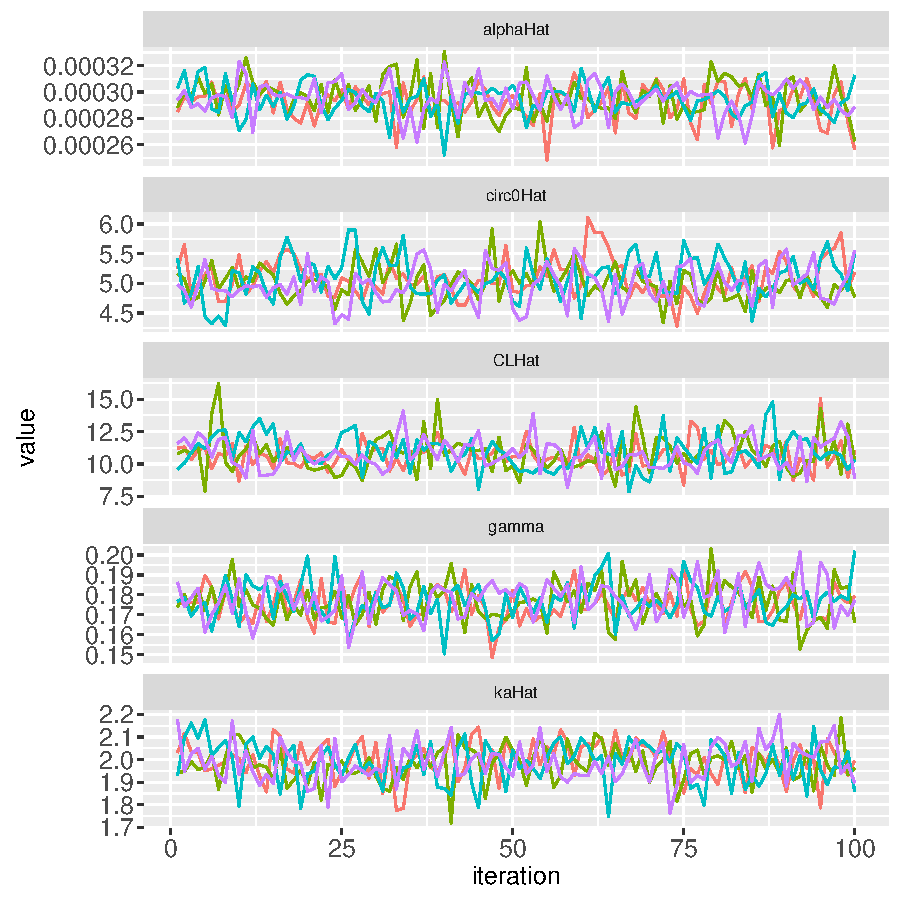
\includegraphics[width=3.0in,trim=0in 0in 0 0in]{graphics/neutropenia/neutropeniaPopulation1TorstenPlots001.pdf}
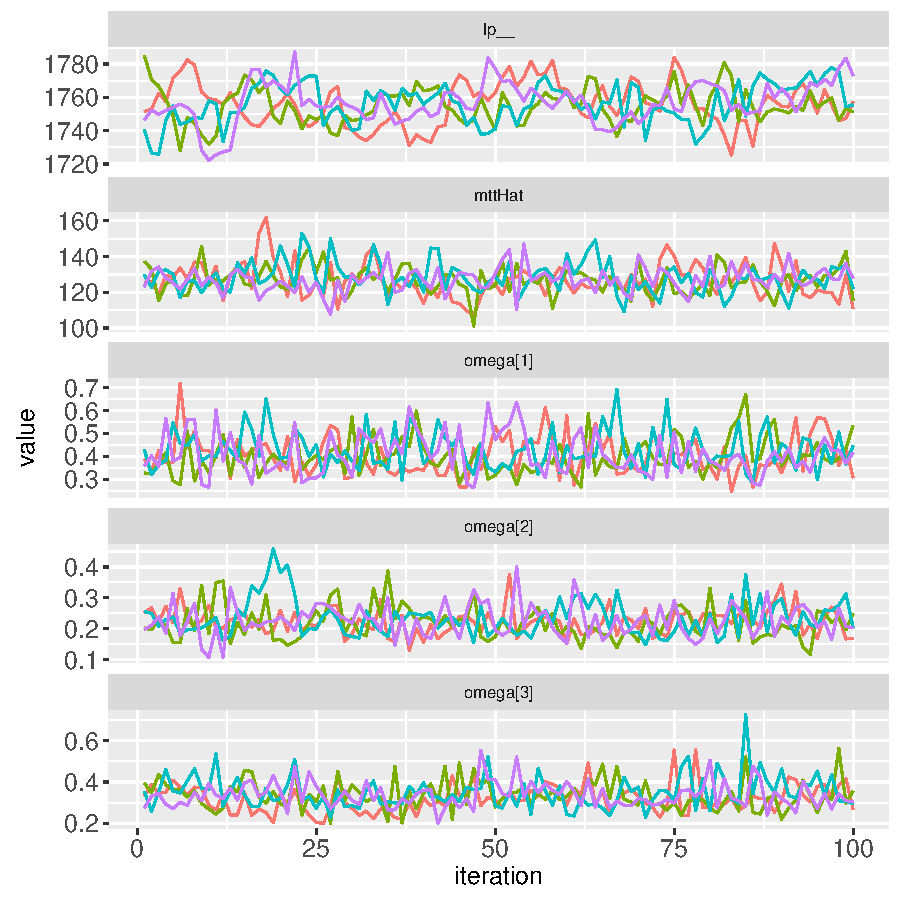
\includegraphics[width=3.0in,trim=0in 0in 0 0in]{graphics/neutropenia/neutropeniaPopulation1TorstenPlots002.pdf}
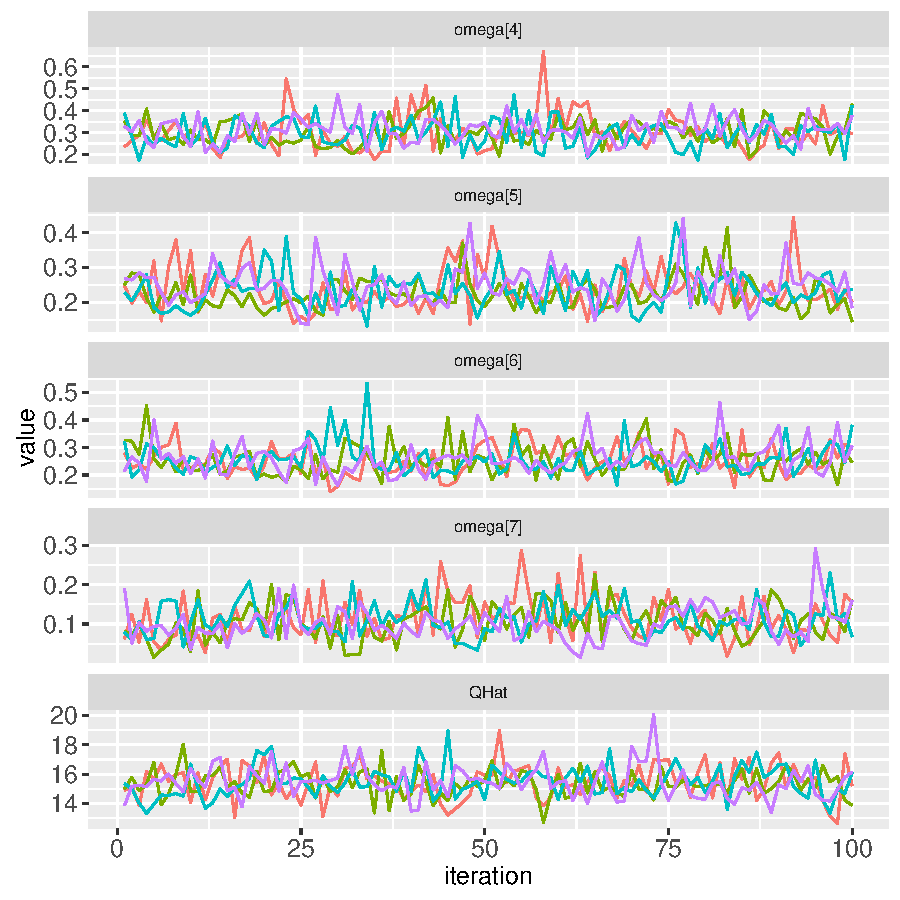
\includegraphics[width=3.0in,trim=0in 0in 0 0in]{graphics/neutropenia/neutropeniaPopulation1TorstenPlots003.pdf}
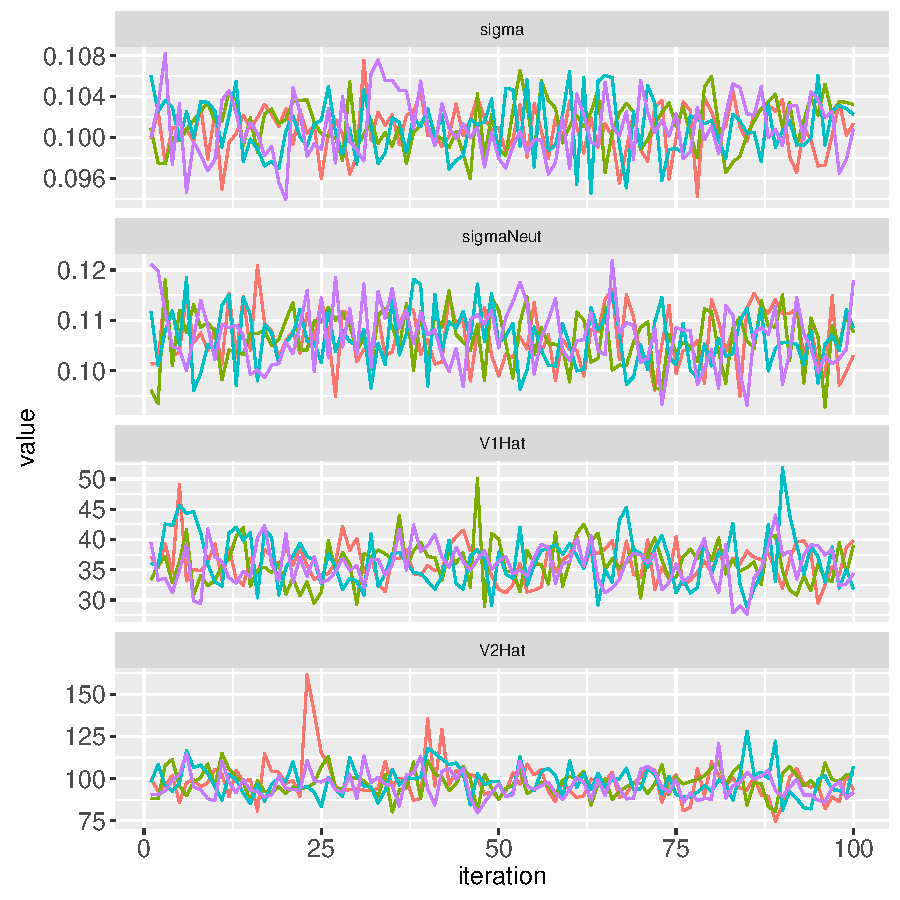
\includegraphics[width=3.0in,trim=0in 0in 0 0in]{graphics/neutropenia/neutropeniaPopulation1TorstenPlots004.pdf}
\caption{{MCMC history plots for the parameters of a Friberg-Karlsson semi-mechanistic model (each color corresponds to a different chain) for example 3}}
\label{FKMCMC}
\end{figure}

\begin{figure}[htbp]
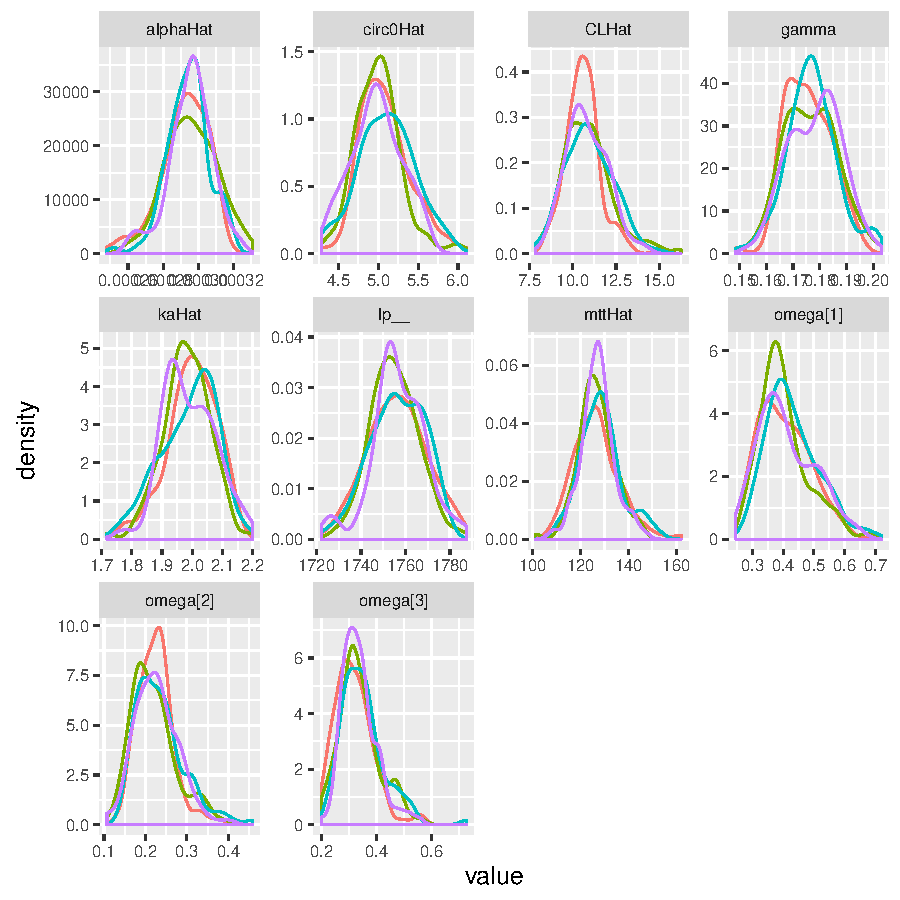
\includegraphics[width=2.5in,trim=0in 0in 0 0in]{graphics/neutropenia/neutropeniaPopulation1TorstenPlots005.pdf}
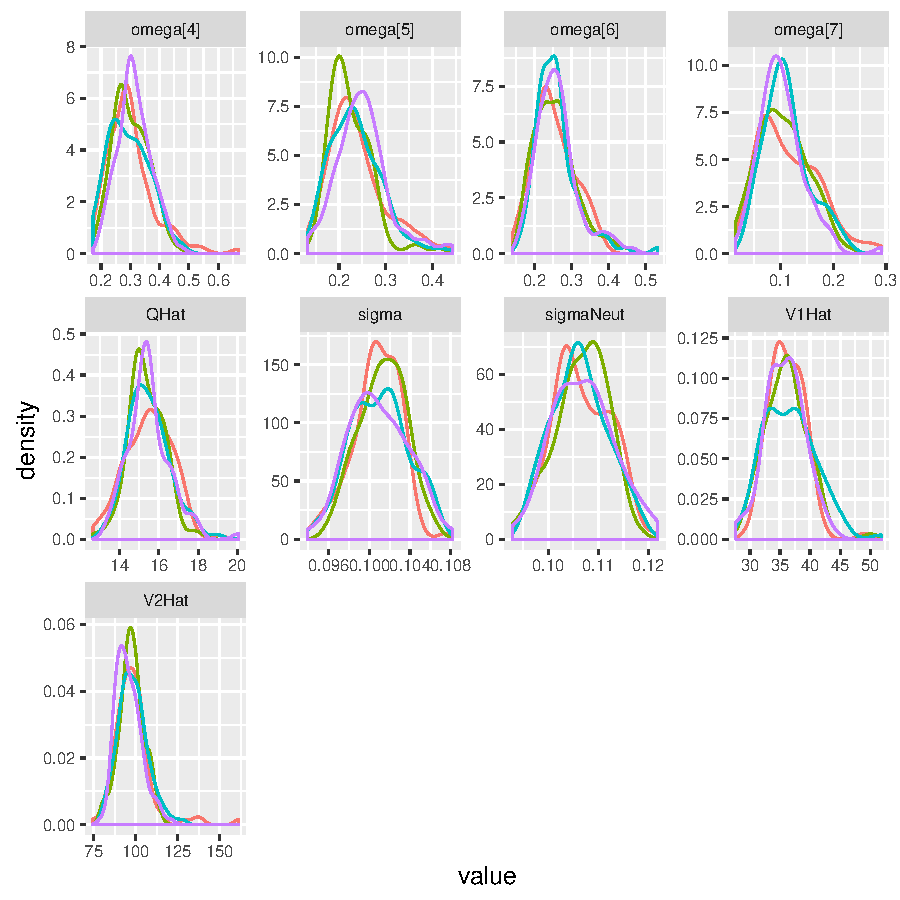
\includegraphics[width=2.5in,trim=0in 0in 0 0in]{graphics/neutropenia/neutropeniaPopulation1TorstenPlots006.pdf}
\caption{{Posterior Marginal Densities of the Model Parameters of a Friberg-Karlsson semi-mechanistic model (each color corresponds to a different chain)}}
\label{FKDens}
\end{figure}

\begin{figure}[htbp]
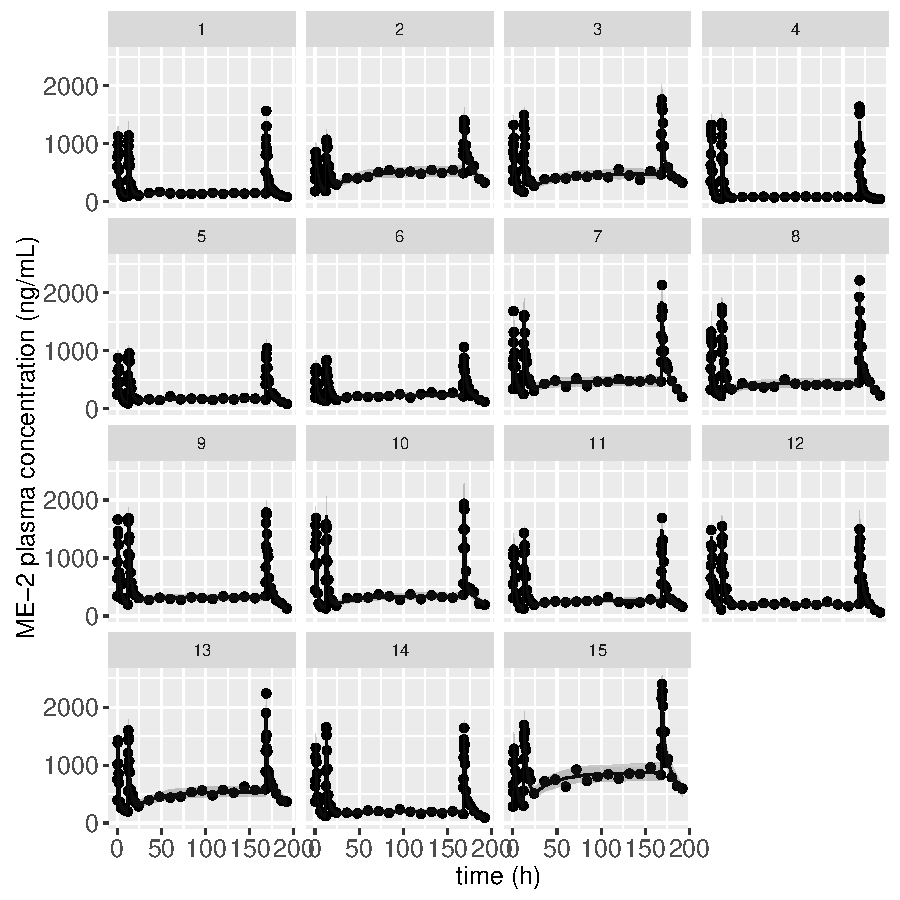
\includegraphics[width=2.5in,trim=0in 0in 0 0in]{graphics/neutropenia/neutropeniaPopulation1TorstenPlots010.pdf}
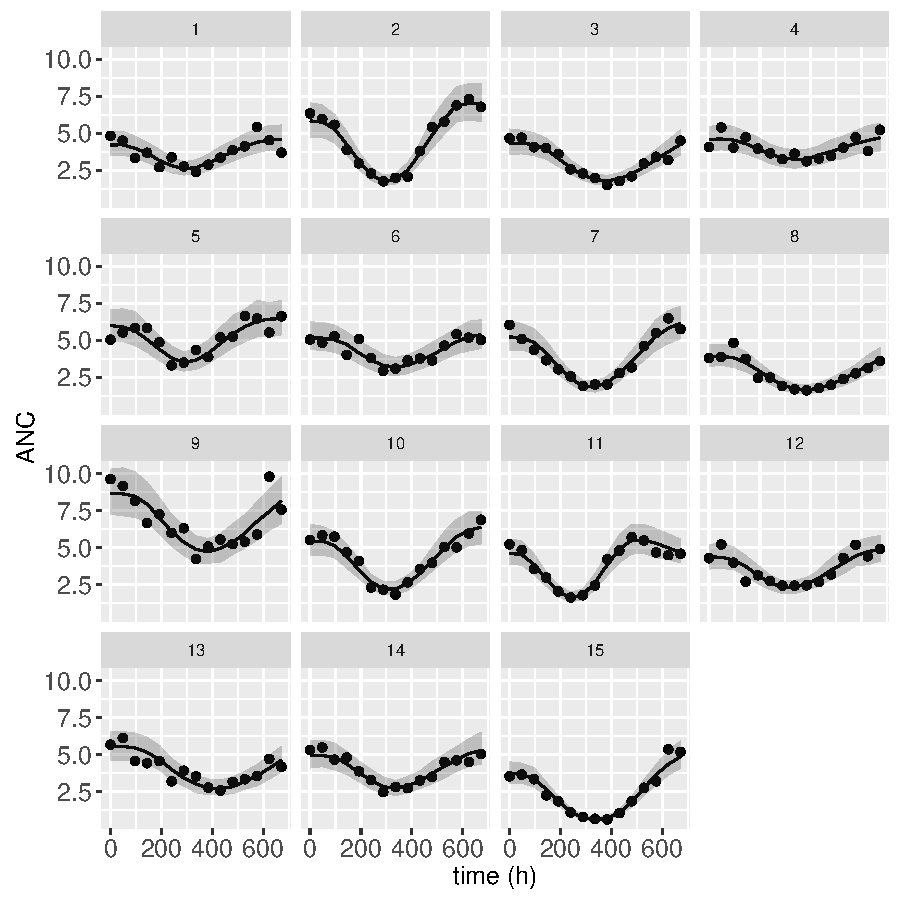
\includegraphics[width=2.5in,trim=0in 0in 0 0in]{graphics/neutropenia/neutropeniaPopulation1TorstenPlots011.pdf}
\caption{{Predicted (posterior median and 90 \% credible intervals) and observed plasma drug concentrations, and Neutrophil counts, for a Friberg-Karlsson semi-mechanistic model}}
\label{FKPredictions}
\end{figure}
 

 
 

\section{Under the Hood Design}
We here discuss some background theory and the design of Torsten at a C++ level.

Our approach is heavily based on the \textit{BUGS model library}, a prototype PKPD model library for WinBUGS (\url{https://bitbucket.org/metrumrg/ bugsmodellibrary/wiki/Home}), developed by Metrum Research Group in 2009.

This section is intended for developers. No knowledge of C++ is required for users.


\subsection{Computing Amounts in an ODE-based model} \ \\ \ \\
Most PKPD model are based on ODEs that describe how PK and PD amounts evolve over time. For instance, the following ODEs describe drug diffusion in a one compartment model with a first-order absorption from the gut:

\begin{eqnarray*}
\frac{dGUT}{dt} &=& -kaGUT \\ 
\frac{dCENT}{dt} &=& kaGUT - \frac{CL}{V_{1}}CENT
\end{eqnarray*}

If the ODEs fully describe the PKPD system, knowing the state $y_0$ at time $t_0$ fully defines the solution at finite times. Exploiting this property, Torsten calculates the evolution of amounts in each compartment from one event to the other. The initial conditions of the ODE system are specified by the previous event, and the ODEs are integrated from $t_{previous} $ to $t_{current}$. 

Note we cannot simply integrate from $t_{first}$ to $t_{last}$ because the ODEs do not describe exterior interventions, such as additional dosing. Torsten treats these interventions independently. Most importantly, Torsten only integrates between $t_0$ and $t_1$ if no exterior interventions occur during this interval. To achieve this, it is key to properly handle the \textit{event schedule}. 

All five functions in Torsten call the C++ function \texttt{pred}, which:
\begin{enumerate}
  \item augments the event schedule to include all events that alter the system
  \item calculates the amounts in each compartment at each event of the augmented schedule by:
  \begin{itemize}
    \item computing the \textit{natural} evolution of the system by integrating ODEs,
    \item or computing alterations due to exterior interventions
  \end{itemize}
  \item returns the amounts at each event of the original schedule
\end{enumerate}

The Event Schedule depends on the user's input (TIME, EVID, CMT, AMT, RATE, ADDL, II, SS). The event schedule may need to be augmented if, for example, an event specifies a patient receives multiple doses at a regular time interval. Consider:

\texttt{TIME = 0, EVID = 1, CMT = 1, AMT = 1500, RATE = 0, ADDL = 4, II = 10, SS = 0} 

This Event specifies that a time 0 (TIME = 0), a patient receives a 1500 mg (AMT = 1500) drug dose (EVID = 1) in the gut (CMT = 1), and will receive an additional dose every 10 hours (II = 10) until the patient has received a total of 5 doses (ADDL = 4, being the number of additional doses, + 1, the original dose). Such an Event really corresponds to 5 dosing events.

To integrate the ODEs, \texttt{pred} calls \texttt{pred1} (prediction for one event) or \texttt{predSS} (prediction for one event if the system is in a steady state, i.e SS = 1). \texttt{pred1} and \texttt{predSS} are functors and get constructed differently by each Torsten function. Under \texttt{PKModelOneCpt}, \texttt{pred1} analytically computes the solution, while under \texttt{generalCptModel\_rk45} it numerically solves the ODEs.
 
\subsection{Structure of a Torsten Function}  \ \\ \ \\
Under the structural scheme described above, a Torsten function performs a very simple set of actions:
\begin{enumerate}
  \item Consistent with Stan practices, check the validity of the arguments and of the parameter values
  \item Construct the PKModel object, which contains basic information about the model, such as the number of compartments
  \item Construct the pred1 and predSS functions
  \item Call pred
\end{enumerate}  

\subsection{Implementing Torsten in Stan}
\subsubsection*{Modifications in Stan-math}
All five Torsten functions are located under the \texttt{Torsten} directory, under \texttt{stan/math}. We modified \texttt{rev/math} to include the \texttt{torsten/torsten.hpp} header file. The code can be found on GitHub: \url{https://github.com/charlesm93/math} 

\subsubsection*{Modifications in Stan}
Further modification are done in Stan to expose the Torsten functions to the Stan language. We edited \texttt{function\_signatures.h} to expose \texttt{PKModelOneCpt}, \texttt{PKModelTwoCpt}, and \texttt{linOdeModel}. The general ODE model functions are higher-order functions (i.e. they take another function as one of their arguments). They were exposed by directly modifying the grammar files, following very closely the example of \texttt{integrate\_ode\_rk45} and \texttt{integrate\_ode\_bdf}.

The code can be found on GitHub:  \url{https://github.com/charlesm93/stan}

\bibliographystyle{custom}
\bibliography{alpha,custom}

%\subsection{Acknowledgments and Thanks}

\end{document}
